\documentclass[xcolor={x11names},10pt]{beamer}

\usetheme{metropolis}
\metroset{numbering=fraction}
\metroset{block=fill}

\newcommand{\backupbegin}{
  \newcounter{finalframe}
  \setcounter{finalframe}{\value{framenumber}}
}
\newcommand{\backupend}{
  \setcounter{framenumber}{\value{finalframe}}
}

\usepackage{headings/kmath}
% Tikz
\usetikzlibrary{calc}
\usetikzlibrary{mindmap,trees,shapes,arrows,backgrounds,topaths}
\usetikzlibrary{decorations.pathmorphing, shapes.geometric}

% Text
\usepackage{enumitem}
\usepackage{ulem}
\usepackage{pifont}

% Maths
\usepackage{amsmath}
\usepackage{amsfonts}
\usepackage{amsthm}
\usepackage{amsopn}

% Plots
\usepackage{pgfplots}
\usepgfplotslibrary{groupplots}

% Tables
\usepackage{booktabs}
\usepackage{array}
\newcolumntype{L}{>$l<$}
\arraycolsep=1.4pt
\setlength{\tabcolsep}{3pt}

% Algos
\usepackage[ruled]{algorithm2e}

% Pgfplot
\pgfplotsset{
    legend image code/.code={
        \draw[mark repeat=2,mark phase=2] plot coordinates {
            (0cm,0cm)
            (0.25cm,0cm)
            (0.25cm,0cm)
        };
    }
}
% Objective values and functions
\newcommand{\pobj}{p}
\newcommand{\robj}{r}

% Variables
\newcommand{\pvletter}{x}
\newcommand{\bvletter}{z}
\newcommand{\pv}{\mathbf{\pvletter}}
\newcommand{\bv}{\mathbf{\bvletter}}
\newcommand{\pvi}[1]{\pvletter_{#1}}
\newcommand{\bvi}[1]{\bvletter_{#1}}

% Problem data
\newcommand{\pdim}{n}
\newcommand{\ddim}{m}
\newcommand{\reg}{\lambda}
\newcommand{\lfunc}{f}
\newcommand{\pfunc}{h}
\newcommand{\rfunc}{g}
\newcommand{\bigM}{M}
\newcommand{\regtwo}{\beta}
\newcommand{\obs}{\mathbf{y}}
\newcommand{\obsi}[1]{y_{#1}}
\newcommand{\dic}{\mathbf{A}}
\newcommand{\noise}{\boldsymbol{\epsilon}}
\newcommand{\groundtruth}{\pv^{\dagger}}

% Indices
\newcommand{\idxentry}{i}

% BnB
\newcommand{\pset}{\mathcal{X}}
\newcommand{\setidx}{\mathcal{S}}
\newcommand{\setzero}{\setidx_0}
\newcommand{\setone}{\setidx_1}
\newcommand{\setnone}{\setidx_\bullet}
\newcommand{\nodeSymb}{\nu}
\newcommand{\node}[1]{#1^{\nodeSymb}}

% Math operators
\DeclareMathOperator{\argmax}{argmax}
\DeclareMathOperator{\argmin}{argmin}
\DeclareMathOperator{\biconjugate}{biconj}
\DeclareMathOperator{\card}{card}
\DeclareMathOperator{\complset}{cmpl}
\DeclareMathOperator{\convex}{cvx}
\DeclareMathOperator{\diam}{diam}
\DeclareMathOperator{\dom}{dom}
\DeclareMathOperator{\interior}{int}
\DeclareMathOperator{\prox}{prox}
\DeclareMathOperator{\rank}{rank}
\DeclareMathOperator{\sign}{sign}


% Math misc
\newcommand{\1}{\mathbf{1}}
\newcommand{\0}{\mathbf{0}}
\newcommand{\abs}[1]{|#1|}
\newcommand{\biconj}[1]{#1^{**}}
\newcommand{\bigO}{\mathcal{O}}
\newcommand{\conj}[1]{#1^{*}}
\newcommand{\icvx}{\text{Ind}}
\newcommand{\intervint}[2]{[#1,#2]}
\newcommand{\iter}[2]{#1^{#2}}
\newcommand{\norm}[2]{\|#1\|_#2}
\newcommand{\opt}[1]{#1^{\star}}
\newcommand{\pospart}[1]{[#1]_+}
\newcommand{\separable}[2]{#1_{#2}}
\newcommand{\subdiff}{\partial}
\newcommand{\transp}[1]{#1^{\mathrm{T}}}

% Edition macros
\newcommand{\AddTodo}[1]{\textcolor{red}{[#1]}}

\newenvironment<>{blockcolor}[2]{%
  \setbeamercolor{block title}{fg=#1,bg=#1!15}%
  \setbeamercolor{block body}{fg=#1,bg=#1!15}%
  \begin{block}#3{\centering#2}
}{%
  \end{block}
}

\definecolor{TolLightWhite}{HTML}{FAFAFA}
\definecolor{TolLightOrange}{HTML}{ECA244}

\begin{document}

\begin{frame}[plain,noframenumbering]
  \begin{tikzpicture}[remember picture,overlay]
    \begin{scope}[xshift=0.5\linewidth]
      \onslide<1-> {
        \node at (0,1) {\large\textbf{Optimization methods for $\boldsymbol{\ell}_{\0}$-problems}};
        %
        \node[text width=\linewidth,align=center] at (0,0) {Théo Guyard \\ {\small{ML MTP -- December 9th, 2024}}};
      }
      %
      %
      %
      % \onslide<2-> {
      %   \node[text width=\linewidth,align=center] at (-3.75,-2.75) {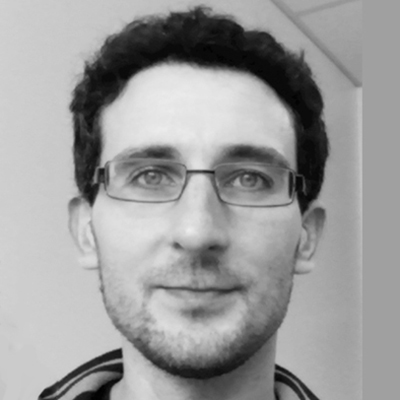
\includegraphics[width=60pt]{imgs/cedric.jpg} \\ \textbf{Cédric Herzet} \\ {\small{Inria/Ensai Rennes}}};
      %   %
      %   \node[text width=\linewidth,align=center] at (0,-2.75) {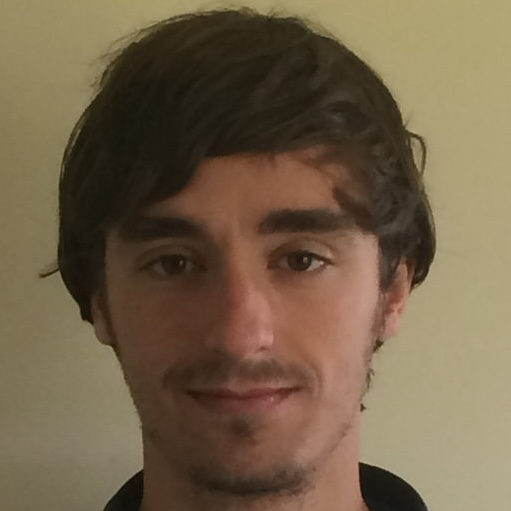
\includegraphics[width=60pt]{imgs/clement.jpg} \\ \textbf{Clément Elvira} \\ {\small{CentraleSupélec Rennes}}};
      %   %
      %   \node[text width=\linewidth,align=center] at (3.75,-2.73) {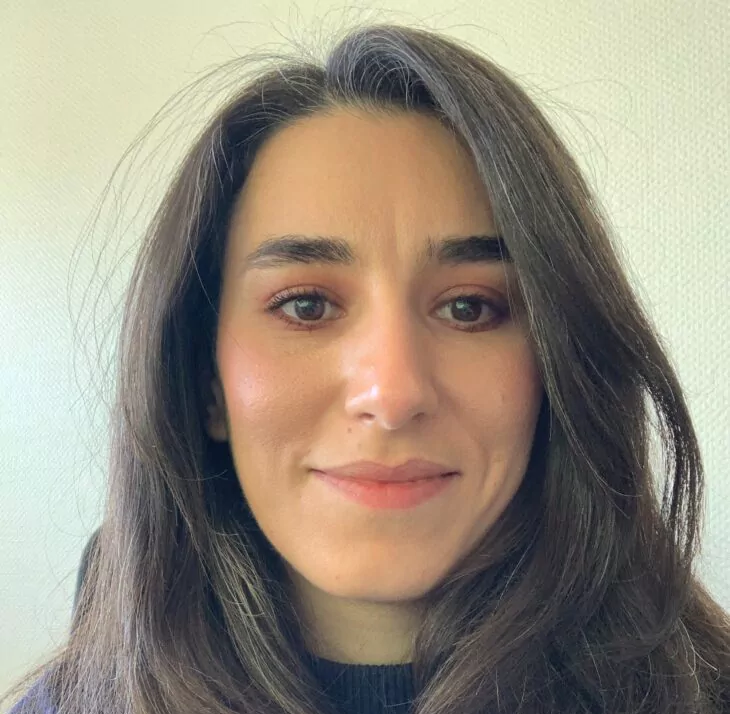
\includegraphics[width=61pt]{imgs/ayse.png} \\ \textbf{Ay\c{s}e-Nur Arslan} \\ {\small{Inria Bordeaux}}};
      % }
    \end{scope}
  \end{tikzpicture}
\end{frame}

\begin{frame}{Sparse optimization}
    \begin{tikzpicture}[remember picture,overlay]
        \begin{scope}[xshift=0.5\textwidth]
            \onslide<1-> {
                \node[text width=0.75\linewidth,align=center] at (0,3.4) {\textbf{Sparse optimization} \\ \textcolor{TolLightOrange}{Minimize} a function with a \textcolor{TolLightOrange}{sparse} solution};
            }
            %
            %
            %
            \onslide<2-> {
                \begin{scope}[yshift=40]
                \path[
                    mindmap,
                    concept color=mDarkTeal, 
                    level 1 concept/.append style={
                    minimum size    = 1.1cm,
                    text width      = 1.1cm,
                    level distance  = 3cm,
                    sibling angle   = 60,
                    font            = \scriptsize\bfseries,
                    },
                    level 2 concept/.append style={
                    minimum size    = 1.1cm,
                    text width      = 1.1cm,
                    level distance  = 2cm,
                    sibling angle   = 45,
                    font            = \scriptsize,
                    }
                ]
                node[concept,text=white,minimum size=1.6cm,text width=2.25cm] {\normalsize\textbf{Applications}}
                [clockwise from=0]
                child[concept color=TolLightRed!40] {
                    node[concept] {signal process.}
                    [clockwise from=45]
                    child { node[concept] {signal denoising} }
                    child { node[concept] {sparse decoding} }
                    child { node[concept] {phase retrieval} }
                    child { node[concept] {DOA design} }
                }  
                child[concept color=TolLightBrown!40] {
                    node[concept] {operation research}
                    [clockwise from=337.5]
                    child { node[concept] {portfolio optim.} }
                    child { node[concept] {network design} }
                    child { node[concept] {facility location} }
                }
                child[concept color=TolLightGreen!40] {
                    node[concept] {algebra}
                    [clockwise from=-67.5]
                    child { node[concept] {sparse factor.} }
                    child { node[concept] {low-rank factor.} }
                    child { node[concept] {feasible system} }
                }
                child[concept color=TolDarkBlue!40] {
                    node[concept] {statistics \& ML} 
                    [clockwise from=-90]
                    child { node[concept] {sparse PCA} }
                    child { node[concept] {sparse SVM} }
                    child { node[concept] {dictionary learning} }
                    child { node[concept] {feature selection} }
                };
                \end{scope}
                %
                \node[font=\small] at (0,-4) {A. Tillmann \textit{et. al} (2024)};
            }
        \end{scope}
    \end{tikzpicture}
\end{frame}
  
\begin{frame}{Compressed sensing}
    \begin{tikzpicture}[remember picture,overlay]
        \begin{scope}[xshift=0.5\textwidth]
            \onslide<1-> {
                \node[text width=0.25\linewidth,align=center] (groundtruth) at (-4,2.5) {Sparse signal \\ $\pv \in \kR^{\pdim}$};
                %
                \draw ($(groundtruth)+(0,-1.75)$) node {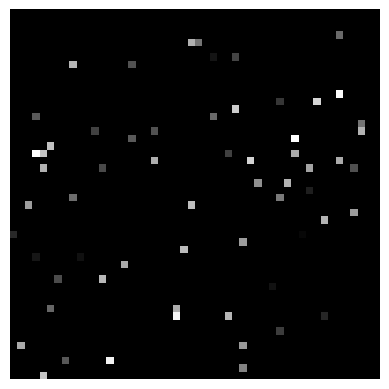
\includegraphics[width=2cm]{imgs/cs-x.png}};
                %
                \node at ($(groundtruth)+(0,-3)$) {$\pdim$ pixels};
            }
            %
            %
            %
            \onslide<2-> {
                \node[text width=0.25\linewidth,align=center] (observation) at (4,2.5) {Observation \\ $\obs = \dic\pv + \boldsymbol{\epsilon} \in \kR^{\ddim}$};
                %
                \draw[ultra thick,->] ($(groundtruth.north east)+(0,-0.25)$) .. controls (0,3.25) .. ($(observation.north west)+(0,-0.25)$) node[midway,fill=TolLightWhite,draw,ultra thick,text width=0.35\linewidth,align=center,yshift=-5] {Linear compression};
                %
                \draw ($(observation)+(0,-1.75)$) node {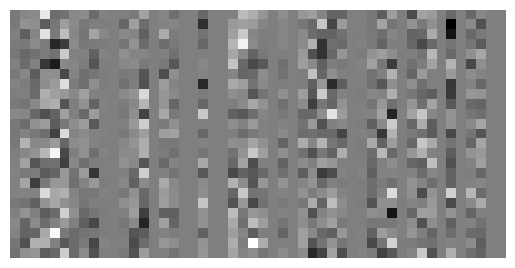
\includegraphics[width=2.5cm]{imgs/cs-y.png}};
                %
                \node at ($(observation)+(0,-2.75)$) {$\ddim$ pixels, $\ddim \ll \pdim$};
            }
            %
            %
            %
            \onslide<3-> {
                \draw[ultra thick,<-] ($(groundtruth.south east)+(0,0.25)$) .. controls (0,1.75) .. ($(observation.south west)+(0,0.25)$) node[midway,fill=TolLightWhite,draw,ultra thick,text width=0.35\linewidth,align=center,yshift=5] {Recover $\pv$ from $\dic$ and $\obs$};
            }
            %
            %
            %
            \onslide<4-> {
                \node [text width=0.45\textwidth] at (0,-1) (problem) {
                    \begin{blockcolor}{mDarkTeal}{Goal}
                    \centering
                    Find $\pv$ such that $\obs \simeq \dic\pv$
                    \end{blockcolor}
                };
            }
            %
            %
            %
            \onslide<5-> {
                \node [text width=0.45\textwidth] at ($(problem)+(0,-2.25)$) (problem-sparse) {
                    \begin{blockcolor}{mDarkTeal}{Goal}
                        \centering
                        Find $\pv$ \textcolor{TolLightOrange}{sparse} such that $\obs \simeq \dic\pv$
                    \end{blockcolor}
                };
                %
                \draw[ultra thick,->] ($(problem)+(0,-0.75)$) -- ($(problem-sparse)+(0,0.5)$) node[midway,fill=TolLightWhite,draw,ultra thick] {no unique solution};
            }
        \end{scope}
    \end{tikzpicture}
\end{frame}
  
\begin{frame}{Feature selection}
    \begin{tikzpicture}[remember picture,overlay]
        \begin{scope}[xshift=0.5\textwidth]
            \onslide<1-> {
                \node (table) at (0,1.5) {
                    \begin{tabular}{c|cccc|c}
                        \toprule
                        & \textbf{Feature 1} & \textbf{Feature 2} & $\quad$...$\quad$ & \textbf{Feature n} & $\ \ $\textbf{Target}$\ \ $ \\
                        \midrule
                        \textbf{Sample 1} & \textcolor{mDarkTeal!20}{$a_{1,1}$} & \textcolor{mDarkTeal!20}{$a_{1,2}$} & \textcolor{mDarkTeal!20}{...} & \textcolor{mDarkTeal!20}{$a_{1,\pdim}$} & \textcolor{mDarkTeal!20}{$\obsi{1}$} \\
                        \textbf{Sample 2} & \textcolor{mDarkTeal!20}{$a_{2,1}$} & \textcolor{mDarkTeal!20}{$a_{2,2}$} & \textcolor{mDarkTeal!20}{...} & \textcolor{mDarkTeal!20}{$a_{2,\pdim}$} & \textcolor{mDarkTeal!20}{$\obsi{2}$} \\
                        \textbf{Sample 3} & \textcolor{mDarkTeal!20}{$a_{3,1}$} & \textcolor{mDarkTeal!20}{$a_{3,2}$} & \textcolor{mDarkTeal!20}{...} & \textcolor{mDarkTeal!20}{$a_{3,\pdim}$} & \textcolor{mDarkTeal!20}{$\obsi{3}$} \\
                        \textcolor{mDarkTeal!20}{...} & \textcolor{mDarkTeal!20}{...} & \textcolor{mDarkTeal!20}{...} & \textcolor{mDarkTeal!20}{...} & \textcolor{mDarkTeal!20}{...} & \textcolor{mDarkTeal!20}{...} \\
                        \textbf{Sample m} & \textcolor{mDarkTeal!20}{$a_{\ddim,1}$} & \textcolor{mDarkTeal!20}{$a_{\ddim,2}$} & \textcolor{mDarkTeal!20}{...} & \textcolor{mDarkTeal!20}{$a_{\ddim,\pdim}$} & \textcolor{mDarkTeal!20}{$\obsi{\ddim}$} \\
                        \bottomrule
                    \end{tabular}
                };
                %
                \node[draw,ultra thick,fill=TolLightWhite,font=\small] (features) at ($(table.center)+(0,-0.5)$) {$\dic \in \kR^{\ddim\times\pdim}$};
                \node[draw,ultra thick,fill=TolLightWhite,font=\small] (outcome) at ($(table.center)+(4.2,-0.5)$) {$\obs \in \kR^{\ddim}$};
            }
            %
            %
            %
            \onslide<2-> {
                \node[text width=0.275\linewidth,align=center] (feature) at ($(table.south)+(-3.5,-0.6)$) {Features $\dic \in \kR^{\ddim\times\pdim}$};
                \node[text width=0.275\linewidth,align=center] (outcome) at ($(table.south)+(3.5,-0.6)$) {Target $\obs = \phi(\dic\pv)$};
                %
                \draw[ultra thick,<->] (feature) -- (outcome) node[midway,below,TolLightOrange] {weights $\pv \in \kR^{\pdim}$};
            }
            %
            %
            %
            \onslide<3-> {
                \node[font=\small,text width=0.3\linewidth,align=center] (loss) at ($(table.south)+(-1.75,-2)$) {\textbf{Model accuracy} \\ Loss $\mathcal{L}_{\phi}(\dic\pv,\obs)$};
                %
                \node[font=\small,text width=0.3\linewidth,align=center] (reg) at ($(table.south)+(1.75,-2)$) {\textbf{Model explicability} \\ Use few features};
            }
            %
            %
            %
            \onslide<4-> {
                \draw[ultra thick,->] (loss) -- ($(loss)+(0,-0.75)$);
                \draw[ultra thick,->] (reg) -- ($(reg)+(0,-0.75)$);
                %
                \node[align=center,text width=0.6\textwidth] (serm) at ($(table.south)+(0,-3.25)$) {
                    \begin{blockcolor}{mDarkTeal}{Goal}
                    \centering
                    Find $\pv$ \textcolor{TolLightOrange}{sparse} such that $\mathcal{L}_{\phi}(\dic\pv,\obs)$ is small 
                    \end{blockcolor}
                };
            }
        \end{scope}
    \end{tikzpicture}
\end{frame}
  
\begin{frame}{Network design}
    \begin{tikzpicture}[remember picture,overlay]
        \begin{scope}[xshift=0.5\textwidth]
        
            \coordinate (A) at (-3.5,1);
            \coordinate (B) at ($(A)+(2,0)$);
            \coordinate (C) at ($(A)+(1,2)$);
            \coordinate (D) at ($(A)+(1,-2)$);
            \coordinate (E) at ($(A)+(3,1)$);
            \coordinate (F) at ($(A)+(3,-1)$);
            \coordinate (G) at ($(A)+(-1,1.5)$);
            \coordinate (H) at ($(A)+(-1,-1.5)$);
            \coordinate (I) at ($(A)+(4,0)$);
            \coordinate (J) at ($(A)+(-2,0)$);

            \draw[ultra thick,dashed] (A) -- (B);
            \draw[ultra thick,dashed] (A) -- (C);
            \draw[ultra thick,dashed] (A) -- (D);
            \draw[ultra thick,dashed] (A) -- (G);
            \draw[ultra thick,dashed] (A) -- (H);
            \draw[ultra thick,dashed] (B) -- (C);
            \draw[ultra thick,dashed] (B) -- (D);
            \draw[ultra thick,dashed] (B) -- (E);
            \draw[ultra thick,dashed] (B) -- (F);
            \draw[ultra thick,dashed] (B) -- (I);
            \draw[ultra thick,dashed] (C) -- (E);
            \draw[ultra thick,dashed] (C) -- (G);
            \draw[ultra thick,dashed] (D) -- (F);
            \draw[ultra thick,dashed] (D) -- (H);
            \draw[ultra thick,dashed] (E) -- (I);
            \draw[ultra thick,dashed] (F) -- (I);
            \draw[ultra thick,dashed] (G) -- (H);
            \draw[ultra thick,dashed] (G) -- (J);
            \draw[ultra thick,dashed] (H) -- (J);

            \node[ultra thick, circle, draw, minimum size=6mm, fill=TolLightWhite] at (A) {};
            \node[ultra thick, circle, draw, minimum size=6mm, fill=TolLightWhite] at (B) {};
            \node[ultra thick, circle, draw, minimum size=6mm, TolLightRed, fill=TolLightWhite] at (C) {\small\textcolor{TolLightRed}{\textbf{3}}};
            \node[ultra thick, circle, draw, minimum size=6mm, TolLightRed, fill=TolLightWhite] at (D) {\small\textcolor{TolLightRed}{\textbf{3}}};
            \node[ultra thick, circle, draw, minimum size=6mm, fill=TolLightWhite] at (E) {};
            \node[ultra thick, circle, draw, minimum size=6mm, fill=TolLightWhite] at (F) {};
            \node[ultra thick, circle, draw, minimum size=6mm, fill=TolLightWhite] at (G) {};
            \node[ultra thick, circle, draw, minimum size=6mm, fill=TolLightWhite] at (H) {};
            \node[ultra thick, circle, draw, minimum size=6mm, TolLightRed, fill=TolLightWhite] at (I) {\small\textcolor{TolLightRed}{\textbf{3}}};
            \node[ultra thick, circle, draw, minimum size=6mm, TolLightBlue, fill=TolLightWhite] at (J) {\small\textcolor{TolLightBlue}{\textbf{9}}};

            \node[text width=0.6\linewidth,align=center] at (-2.5,-2) {Which edges to build to transport products from \textcolor{TolLightBlue}{source} to \textcolor{TolLightRed}{sink} nodes ?};


            \node[ultra thick, circle, draw, minimum size=6mm, fill=TolLightWhite] (N1) at (2.5,1) {};
            \node[ultra thick, circle, draw, minimum size=6mm, fill=TolLightWhite] (N2) at (4.5,1) {};
            \draw[ultra thick,dashed] (N1) -- (N2);
            \node[text width=0.5\linewidth,align=center,anchor=north] at ($(N1)!0.5!(N2)+(0,-0.5)$) {construction cost $c$ per edge \\ transportation cost $Q(\pv)$ \\ capacity $\0 \leq \pv \leq \mathbf{x}_{\text{ub}}$ \\ flow conservation $\mathbf{D}\pv \leq \mathbf{d}$};

            % \node[text width=0.35\linewidth,align=center] at (9,1) {
            %   \begin{blockcolor}{mDarkTeal}{Network design}
            %       \centering
            %       $\textstyle
            %       \left\{
            %           \begin{array}{rl}
            %               \min & Q(\pv) + \reg\norm{\pv}{0} \\ 
            %               \text{s.t.} & \mathbf{D}\pv \leq \mathbf{d}, \ \pv \leq \mathbf{c} \\ & \pv \in \kR+^{\card(E)}
            %           \end{array}
            %       \right.$
            %   \end{blockcolor}
            % };
            % \node[text width=0.5\linewidth,align=left] at (10.5,-2) {\begin{itemize}[nosep]\item[$Q$ :] transportation cost \item[$\reg$ :] unit construction cost \item[$\mathbf{D}\pv \leq \mathbf{d}$ :] flow conservation \item[$\0 \leq \pv \leq \mathbf{c}$ :] capacity constraint\end{itemize}};
        \end{scope}
    \end{tikzpicture}
\end{frame}
  
\begin{frame}{Minimized, constrained, or regularized problem ?}
    \begin{tikzpicture}[remember picture,overlay]
        \begin{scope}[xshift=0.5\textwidth]
            \onslide<1-> {
                \node[text width=0.75\linewidth,align=center] (sparse) at (0,3.4) {\textbf{Sparse optimization} \\ \textcolor{TolLightOrange}{Minimize} a function with a \textcolor{TolLightOrange}{sparse} solution};
            }
            %
            %
            %
            \onslide<2-> {
                \node[text width=0.35\textwidth,align=center] (loss) at (-3,1) {$\lfunc(\pv)$ \\ thing to minimize};
                %
                % \draw[ultra thick] ($(sparse)+(-3.2,-0.4)$) -- ($(sparse)+(-3.2,-0.5)$) -- ($(sparse)+(-0.15,-0.5)$) -- ($(sparse)+(-0.15,-0.4)$);
                %
                \draw [ultra thick,->] ($(sparse)+(-1.5,-0.5)$) -- (loss) node[midway,fill=TolLightWhite,draw,ultra thick] {quantify cost};
            }
            %
            %
            %
            \onslide<3-> {
                \node[text width=0.35\textwidth,align=center] (norm) at (3,1) {$\norm{\pv}{0}$ \\ counts non-zeros};
                %
                % \draw[ultra thick] ($(sparse)+(3.2,-0.4)$) -- ($(sparse)+(3.2,-0.5)$) -- ($(sparse)+(0.9,-0.5)$) -- ($(sparse)+(0.9,-0.4)$);
                %
                \draw [ultra thick,->] ($(sparse)+(1.5,-0.5)$) -- (norm) node[midway,fill=TolLightWhite,draw,ultra thick] {quantify sparsity};
            }
            %
            %
            %
            \onslide<4-> {
                \node[text width=0.45\textwidth] at (-3,-1) {
                \begin{blockcolor}{mDarkTeal}{\textbf{Constrained version}}
                    \centering
                    $\begin{array}{ll} \min_{\pv \in \kR^{\pdim}} & \ \lfunc(\pv) \\ \text{subject to} & \ \norm{\pv}{0} \leq s\end{array}$
                \end{blockcolor}
                };
            }
            %
            %
            %
            \onslide<5-> {
                \node[text width=0.45\textwidth] at (3,-1) {
                \begin{blockcolor}{mDarkTeal}{\textbf{Minimized version}}
                    \centering
                    $\begin{array}{ll} \min_{\pv \in \kR^{\pdim}} & \ \norm{\pv}{0} \\ \text{subject to} & \ \lfunc(\pv) \leq \epsilon\end{array}$
                \end{blockcolor}
                };
            }
            %
            %
            %
            \onslide<6-> {
                \node[text width=0.45\textwidth] at (0,-3.25) {
                \begin{blockcolor}{mDarkTeal}{\textbf{Regularized version}}
                    \centering
                    $\min_{\pv \in \kR^{\pdim}} \lfunc(\pv) + \reg\norm{\pv}{0} + \textcolor{TolLightOrange}{\pfunc(\pv)}$
                \end{blockcolor}
                };
            }
        \end{scope}
    \end{tikzpicture}
\end{frame}
  
\begin{frame}{A bit of history}
    \begin{tikzpicture}[remember picture,overlay]
        \begin{scope}[xshift=0.5\textwidth]
            \onslide<1-> {
                \node[align=center,text width=0.45\textwidth] (problem) at (0,3) {
                    \begin{blockcolor}{mDarkTeal}{Problem}
                        \centering
                        $\min_{\pv \in \kR^{\pdim}} \lfunc(\pv) + \reg\norm{\pv}{0} + \pfunc(\pv)$
                    \end{blockcolor}
                };
                %
                \node at ($(problem.south)+(0,-0.1)$) {NP-hard to solve};
            }
            %
            %
            %
            \onslide<2-> {
                \node (linecenter) at ($(current page.north)+(0,-0.55\textheight)$) {};
                \draw [ultra thick,->] ($(linecenter)+(-6,0)$) -- ($(linecenter)+(6,0)$) node (arrow) [midway] {};
                %
                \node (date1) at ($(linecenter)+(-5,0)$) {};
                \draw [ultra thick,-] ($(date1)+(0,-0.02\textheight)$) -- ($(date1)+(0,0.02\textheight)$);
                \node at ($(date1)+(0,+0.06\textheight)$)  {\textbf{1995}};
                \node[text width=0.2\textwidth,align=center,font=\small] at ($(date1)+(0,-0.05\textheight)$) {Heuristics};
                \node[text width=0.3\textwidth,align=center,font=\scriptsize] at ($(date1)+(0,-0.12\textheight)$) {MP, OMP, ... \\ S. Mallat (1993)};
                %
                \node (origin1) at ($(date1)+(0,-0.4\textheight)$) {};
                \fill[draw,thick,fill=TolLightWhite] ($(origin1)+(-0.5,0)$) circle (0.1);
                \fill[draw,thick,fill=TolLightOrange] ($(origin1)+(-0.5,0.3)$) circle (0.1);
                \fill[draw,thick,fill=TolLightWhite] ($(origin1)+(-0.5,0.6)$) circle (0.1);
                \fill[draw,thick,fill=TolLightWhite] ($(origin1)+(-0.5,0.9)$) circle (0.1);
                \fill[draw,thick,fill=TolLightWhite] ($(origin1)+(-0.5,1.2)$) circle (0.1);
                \fill[draw,thick,fill=TolLightWhite] ($(origin1)+(-0.5,1.5)$) circle (0.1);
                \node at ($(origin1)+(-0.5,-0.4)$) {$\pv^1$};
                %
                \fill[draw,thick,fill=TolLightWhite] ($(origin1)+(0,0)$) circle (0.1);
                \fill[draw,thick,fill=TolLightOrange] ($(origin1)+(0,0.3)$) circle (0.1);
                \fill[draw,thick,fill=TolLightWhite] ($(origin1)+(0,0.6)$) circle (0.1);
                \fill[draw,thick,fill=TolLightOrange] ($(origin1)+(0,0.9)$) circle (0.1);
                \fill[draw,thick,fill=TolLightWhite] ($(origin1)+(0,1.2)$) circle (0.1);
                \fill[draw,thick,fill=TolLightWhite] ($(origin1)+(0,1.5)$) circle (0.1);
                \node at ($(origin1)+(0,-0.4)$) {$\pv^2$};
                %
                \fill[draw,thick,fill=TolLightWhite] ($(origin1)+(0.5,0)$) circle (0.1);
                \fill[draw,thick,fill=TolLightOrange] ($(origin1)+(0.5,0.3)$) circle (0.1);
                \fill[draw,thick,fill=TolLightWhite] ($(origin1)+(0.5,0.6)$) circle (0.1);
                \fill[draw,thick,fill=TolLightOrange] ($(origin1)+(0.5,0.9)$) circle (0.1);
                \fill[draw,thick,fill=TolLightOrange] ($(origin1)+(0.5,1.2)$) circle (0.1);
                \fill[draw,thick,fill=TolLightWhite] ($(origin1)+(0.5,1.5)$) circle (0.1);
                \node at ($(origin1)+(0.5,-0.4)$) {$\pv^3$};
            }
            %
            %
            %
            \onslide<3-> {
                \node (date2) at ($(linecenter)+(-2.5,0)$) {};
                \draw [ultra thick,-] ($(date2)+(0,-0.02\textheight)$) -- ($(date2)+(0,0.02\textheight)$);
                \node at ($(date2)+(0,+0.06\textheight)$)  {\textbf{2000}};
                \node[text width=0.25\textwidth,align=center,font=\small] at ($(date2)+(0,-0.053\textheight)$) {Recovery cond.};
                \node[text width=0.3\textwidth,align=center,font=\scriptsize] at ($(date2)+(0,-0.12\textheight)$) {RIP, NSP, ... \\ E. Candes (2004)};
                %
                \node (origin2) at ($(date2)+(0,-0.4\textheight)$) {};
                \node[text width=0.2\linewidth,align=center,font=\small] at ($(origin2)+(0,0.065\textheight)$) {OMP solves $\ell_0$-problem under RIP};
            }
            %
            %
            %
            \onslide<4-> {
                \node (date3) at ($(linecenter)+(0,0)$) {};
                \draw [ultra thick,-] ($(date3)+(0,-0.02\textheight)$) -- ($(date3)+(0,0.02\textheight)$);
                \node at ($(date3)+(0,+0.06\textheight)$)  {\textbf{2005}};
                \node[font=\small] at ($(date3)+(0,-0.053\textheight)$) {Convex approx.};
                \node[text width=0.3\textwidth,align=center,font=\scriptsize] at ($(date3)+(0,-0.12\textheight)$) {Lasso, Elastic-Net, ... \\ R. Tibshirani (2005)};
                %
                \node (origin3) at ($(date3)+(0,-0.4\textheight)$) {};
                \draw[ultra thick,->] ($(origin3)+(-1,0)$) -- ($(origin3)+(1, 0)$);
                \draw[ultra thick,->] ($(origin3)+(0,0)$) -- ($(origin3)+(0,1.5)$);
                \draw[-,very thick,TolLightOrange] ($(origin3)+(-0.05,0.8)$) -- ($(origin3)+(-1,0.8)$);
                \draw[-,very thick,TolLightOrange] ($(origin3)+(0.05,0.8)$) -- ($(origin3)+(1,0.8)$);
                \draw[very thick,dashed,TolLightOrange] (origin3) .. controls ($(origin3)+(-0.5,0.1)$) ..  ($(origin3)+(-1,0.8)$);
                \draw[very thick,dashed,TolLightOrange] (origin3) .. controls ($(origin3)+(0.5,0.1)$) ..  ($(origin3)+(1,0.8)$);
                \draw[TolLightOrange,very thick] ($(origin3)+(0,0.8)$) circle (0.075);
                \fill[TolLightOrange] (origin3) circle (0.075);
            }
            %
            %
            %
            \onslide<5-> {
                \node (date4) at ($(linecenter)+(2.5,0)$) {};
                \draw [ultra thick,-] ($(date4)+(0,-0.02\textheight)$) -- ($(date4)+(0,0.02\textheight)$);
                \node at ($(date4)+(0,+0.06\textheight)$)  {\textbf{2010}};
                \node[font=\small] at ($(date4)+(0,-0.053\textheight)$) {Concave approx.};
                \node[text width=0.3\textwidth,align=center,font=\scriptsize] at ($(date4)+(0,-0.12\textheight)$) {SCAD, MCP, ... \\ C. Zhang (2010)};
                %
                \node (origin4) at ($(date4)+(0,-0.4\textheight)$) {};
                \draw[ultra thick,->] ($(origin4)+(-1,0)$) -- ($(origin4)+(1, 0)$);
                \draw[ultra thick,->] ($(origin4)+(0,0)$) -- ($(origin4)+(0,1.5)$);
                \draw[-,very thick,TolLightOrange] ($(origin4)+(-0.05,0.8)$) -- ($(origin4)+(-1,0.8)$);
                \draw[-,very thick,TolLightOrange] ($(origin4)+(0.05,0.8)$) -- ($(origin4)+(1,0.8)$);
                \draw[very thick,TolLightOrange,dashed] (origin4) .. controls ($(origin4)+(-0.5,0.8)$) ..  ($(origin4)+(-1,0.8)$);
                \draw[very thick,TolLightOrange,dashed] (origin4) .. controls ($(origin4)+(0.5,0.8)$) ..  ($(origin4)+(1,0.8)$);
                \draw[TolLightOrange,very thick] ($(origin4)+(0,0.8)$) circle (0.075);
                \fill[TolLightOrange] (origin4) circle (0.075);
            }
            %
            %
            %
            \onslide<6-> {
                \node (date5) at ($(linecenter)+(5,0)$) {};
                \draw[ultra thick,-] ($(date5)+(0,-0.02\textheight)$) -- ($(date5)+(0,0.02\textheight)$);
                \node at ($(date5)+(0,+0.06\textheight)$)  {\textbf{2015}};
                \node[text width=0.22\textwidth,align=center,font=\small,TolLightOrange] at ($(date5)+(0,-0.05\textheight)$) {Exact methods};
                \node[text width=0.3\textwidth,align=center,font=\scriptsize] at ($(date5)+(0,-0.12\textheight)$) {MIP, BnB, ... \\ D. Bertsimas (2016)};
                %
                \node (origin5) at ($(date5)+(0,-0.4\textheight)$) {};
                \draw[ultra thick,->] ($(origin5)+(-1,0)$) -- ($(origin5)+(1, 0)$);
                \draw[ultra thick,->] ($(origin5)+(0,0)$) -- ($(origin5)+(0,1.5)$);
                \draw[-,very thick,TolLightOrange] ($(origin5)+(-0.05,0.8)$) -- ($(origin5)+(-1,0.8)$);
                \draw[-,very thick,TolLightOrange] ($(origin5)+(0.05,0.8)$) -- ($(origin5)+(1,0.8)$);
                \draw[TolLightOrange,very thick] ($(origin5)+(0,0.8)$) circle (0.075);
                \fill[TolLightOrange] (origin5) circle (0.075);
            }
        \end{scope}
    \end{tikzpicture}
\end{frame}
  
\begin{frame}{Complexity-tractability balance}
    \AddTodo{Slide, tell what's my point with this talk}
\end{frame}
\section{Mixed-Integer Programming}

\begin{frame}{MIP -- Pipeline}
    \begin{tikzpicture}[remember picture,overlay]
        \begin{scope}[xshift=0.5\textwidth]
            \onslide<1-> {
                \node[text width=0.75\linewidth, align=center] (application) at (-2,3.25) {\textbf{Application} \\ {\small{ML, Stats, Signal, Operation Research, ...}}};
                %
                \node[align=center,text width=0.45\textwidth] (problem) at ($(application)+(0,-1.5)$) {
                    \begin{blockcolor}{mDarkTeal}{Problem}
                    \centering
                    $\min_{\pv \in \kR^{\pdim}} \lfunc(\pv) + \reg\norm{\pv}{0} + \pfunc(\pv)$
                    \end{blockcolor}
                };
                \draw[->,ultra thick] (application) -- ($(problem)+(0,0.6)$);
            }
            %
            %
            %
            \onslide<2-> {
                \node[align=center,text width=0.45\textwidth] (formulation) at ($(problem)+(0,-2.75)$) {
                    \begin{blockcolor}{mDarkTeal}{MIP formulation}
                    \centering
                    Standardized expressions
                    \end{blockcolor}
                };
                \draw[->,ultra thick] (problem) -- ($(formulation)+(0,0.6)$);
            }
            %
            %
            %
            \onslide<3-> {
                \node (middle-problem-formulation) at ($(problem)!0.5!(formulation)+(0,-0.05)$) {};
                \node[align=center,text width=0.375\textwidth,font=\small] (framework) at ($(middle-problem-formulation)+(5,0)$) {\textbf{Modelling framework} \\ $\begin{array}{rcl} \text{Python} & \rightarrow &  \texttt{cvxpy} \\ \text{Julia} & \rightarrow &  \texttt{JuMP} \\ \text{C++} & \rightarrow &  \texttt{CMPL} \\ \text{Matlab} & \rightarrow &  \texttt{YALMIP} \\ & ... & \end{array}$};
                \fill[draw,thick,fill=mDarkTeal] (middle-problem-formulation) circle (0.075);
                \draw[->,ultra thick,dashed] (middle-problem-formulation) -- ($(framework)+(-1.75,0)$);
            }
            %
            %
            %
            \onslide<4-> {
                \node[align=center,text width=0.425\textwidth,fill=mDarkTeal!15] (solution) at ($(formulation)+(0,-2.5)$) {\textbf{Problem solutions}};
                \draw[->,ultra thick] (formulation) -- ($(solution)+(0,0.4)$);
            }
            %
            %
            %
            \onslide<5-> {
                \node (middle-formulation-solution) at ($(formulation)!0.5!(solution)+(0,-0.15)$) {};
                \node[align=center,text width=0.375\textwidth,font=\small] (solver) at ($(middle-formulation-solution)+(5,0)$) {\textbf{Generic MIP solver} \\ Gurobi, CPLEX, SCIP, \\ Mosek, CbC, ...};
                \fill[draw,thick,fill=mDarkTeal] (middle-formulation-solution) circle (0.075);
                \draw[->,ultra thick,dashed] (middle-formulation-solution) -- ($(solver)+(-1.75,0)$);
            }
        \end{scope}
    \end{tikzpicture}
\end{frame}

\begin{frame}{MIP -- Formulation}
    \begin{tikzpicture}[remember picture,overlay]
        \begin{scope}[xshift=0.5\textwidth]
            \onslide<1-> {
                \node[align=center,text width=0.5\textwidth] (problem) at (-2.75,3.25) {
                    \begin{blockcolor}{mDarkTeal}{Problem}
                    \centering
                    $\min_{\pv \in \kR^{\pdim}} \lfunc(\pv) + \reg\norm{\pv}{0} + \pfunc(\pv)$
                    \end{blockcolor}
                };
                %
                \node[text width=0.55\linewidth,align=center,font=\small] at ($(problem)+(5.75,-0.15)$) {\textbf{MIP formulation} \\ Use standardized expressions \\ linear, quadratic, conic, ...};
            }
            %
            %
            %
            \onslide<2-> {
                \node[align=center,text width=0.5\textwidth] (mip) at ($(problem)+(0,-2.9)$) {
                    \begin{blockcolor}{mDarkTeal}{Lifted formulation}
                    \centering
                    $\left\{\begin{array}{rcl}\min && \lfunc(\pv) + \reg\textcolor{TolLightOrange}{\transp{\1}\bv} + \pfunc(\pv) \\
                    \text{s.t.} && \textcolor{TolLightOrange}{\pvi{\idxentry} = 0 \implies \bvi{\idxentry} = 0, \ \forall \idxentry} \\
                    && \pv \in \kR^{\pdim}, \ \textcolor{TolLightOrange}{\bv \in \{0,1\}^{\pdim}}\end{array}\right.$
                    \end{blockcolor}
                };
                %
                \node[text width=0.525\linewidth,align=center,font=\small] at ($(mip)+(5.75,-0.15)$) {\textbf{Lifted $\boldsymbol{\ell}_{\0}$-norm formulation} \\ $\norm{\pv}{0}$ $=$ $\transp{\1}\bv$ with $\pv \in \kR^{\pdim}$ and $\bv \in \{0,1\}^{\pdim}$ \\ if $\pvi{\idxentry} = 0$ $\iff$ $\bvi{\idxentry} = 0$ for all $\idxentry \in \intervint{1}{\pdim}$};
                %
                \draw[ultra thick,->] (problem) -- ($(mip.north)+(0,-0.25)$) node[midway,font=\small,fill=TolLightWhite,draw,ultra thick,yshift=1.5pt] {linearize $\ell_0$-norm};
            }
            %
            %
            %
            \onslide<3-> {
                \node[align=center,text width=0.5\textwidth] (practical-mip) at ($(mip)+(0,-3.25)$) {
                    \begin{blockcolor}{mDarkTeal}{MIP formulation}
                    \centering
                    $\left\{\begin{array}{rcl}\min && \lfunc(\pv) + \reg\transp{\1}\bv + \textcolor{TolLightOrange}{\pfunc_{\text{mip}}(\pv,\bv)} \\
                    \text{s.t.} && \pv \in \kR^{\pdim}, \ \bv \in \{0,1\}^{\pdim}\end{array}\right.$
                    \end{blockcolor}
                };
                %
                \draw[ultra thick,->] (mip) -- ($(practical-mip.north)+(0,-0.25)$) node[midway,font=\small,fill=TolLightWhite,draw,ultra thick,yshift=1.5pt] {avoid logical cstr.};
                %
                \node[text width=0.525\linewidth,align=center,font=\small] at ($(practical-mip)+(5.75,-0.15)$) {
                    \textbf{Logical constraint standardization} \\[0.5em]
                    {
                        \scriptsize
                        $\begin{array}{ll}
                        \toprule
                        \pfunc(\pv) & \pfunc_{\text{mip}}(\pv,\bv) \\ \midrule
                        \icvx(\norm{\pv}{\infty} \leq \bigM) \quad~ & \icvx(-\bigM \bv \leq \pv \leq \bigM \bv) \\
                        \regtwo\norm{\pv}{2}^2 & \sum_{\idxentry=1}^{\pdim} \regtwo\tfrac{\pvi{\idxentry}^2}{\bvi{\idxentry}} \\ 
                        \bottomrule
                        \end{array}$
                    }
                };
            }
        \end{scope}
    \end{tikzpicture}
\end{frame}

\begin{frame}[fragile]{MIP -- Hands-on with \texttt{cvxpy}}
    \begin{tikzpicture}[remember picture,overlay]
        \begin{scope}[xshift=0.5\linewidth]
            \node[text width=0.4\linewidth,align=center] (reg) at (-3.5,2.75) {\textbf{Sparse regression} \\ Find $\pv$ sparse such that $\obs \simeq \dic\pv$};
            %
            \node[text width=0.6\linewidth,align=center] (opt) at ($(reg)+(0,-2)$) {\textbf{Optimization problem} \\ $\min_{\pv \in \kR^{\pdim}} \lfunc(\pv) + \reg\norm{\pv}{0} + \pfunc(\pv)$};
            %
            \node[text width=0.45\linewidth,align=center] at ($(opt)+(0,-1)$) {
                \begin{itemize}[label=\textbullet,nosep]
                \item $\lfunc(\pv) = \tfrac{1}{2}\norm{\obs - \dic\pv}{2}^2$
                \item $\pfunc(\pv) = \icvx(-\bigM \leq \pv \leq \bigM)$
                \end{itemize}
            };
            %
            \draw[ultra thick,->] (reg) -- (opt);
            %
            \node[text width=0.6\linewidth,align=center] (mip) at ($(opt)+(0,-3.5)$) {\textbf{MIP formulation} \\[0.5em] $\left\{\begin{array}{ll}\min &\lfunc(\pv) + \reg\transp{\1}\bv \\ \text{s.t.} & -\bigM\bv \leq \pv \leq \bigM\bv \\ & \pv \in \kR^{\pdim}, \bv \in \{0,1\}^{\pdim} \end{array}\right.$};
            %
            \draw[ultra thick,->] ($(opt)+(0,-1.75)$) -- (mip);
            %
            \node[fill=mDarkTeal] at (2.5,3.5) {\textcolor{TolLightWhite}{\texttt{\$ pip install cvxpy}}};
            %
            \node[text width=0.9\linewidth,align=center] at (2.5,-0.5) {
                \begin{lstlisting}
                import cvxpy as cp
                from sklearn.datasets import make_regression
                
                # Generate sparse regression data
                A, y = make_regression()
                
                # Define variables
                n = A.shape[1]
                x = cp.Variable(n)
                z = cp.Variable(n, boolean=True)

                # Define objective and constraints
                objective = cp.Minimize(
                    cp.sum_squares(A @ x - y) + 10 * cp.sum(z)
                )
                constraints = [-M * z <= x, x <= M * z]

                # Solve the problem using Gurobi
                problem = cp.Problem(objective, constraints)
                problem.solve(solver=cp.GUROBI)
                \end{lstlisting}
            };
        \end{scope}
    \end{tikzpicture}
\end{frame}

\begin{frame}{MIP -- Let's sum up}
    \begin{tikzpicture}[remember picture,overlay]
        \begin{scope}[xshift=0.5\textwidth]
            \node[align=center,text width=0.425\textwidth] (problem) at (0,3) {
                \begin{blockcolor}{mDarkTeal}{Problem}
                    \centering
                    $\min_{\pv \in \kR^{\pdim}} \lfunc(\pv) + \reg\norm{\pv}{0} + \pfunc(\pv)$
                \end{blockcolor}
            };
            %
            \node[text width=0.425\linewidth,align=center] at ($(problem)+(0,-2.25)$) {
                \centering
                \textbf{Pipeline} \\
                \begin{enumerate}[label=\textbf{\arabic*)}]
                \item Introduce binary variable
                \item Establish MIP formulation
                \item Use generic MIP solvers
                \end{enumerate}
            };
            %
            \node[align=center,text width=0.475\textwidth] (problem) at (-3,-2.25) {
                \begin{blockcolor}{TolLightGreen}{Pros}
                \centering
                \begin{itemize}[label=\ding{51}]
                    \item Rich MIP literature
                    \item Black-box solvers
                    \item Convenient for practitioners
                \end{itemize}
                \end{blockcolor}
            };
            %
            \node[align=center,text width=0.475\textwidth] (problem) at (3,-2.25) {
                \begin{blockcolor}{TolLightRed}{Cons}
                \centering
                \begin{itemize}[label=\ding{55}]
                    \item Mostly commercial solvers
                    \item Unable to exploit structure
                    \item Performance issues
                \end{itemize}
                \end{blockcolor}
            };
        \end{scope}
    \end{tikzpicture}
\end{frame}

\section{Branch-and-Bound Algorithms}

\begin{frame}{BnB -- Pipeline}
    \begin{tikzpicture}[remember picture,overlay]
        \begin{scope}[xshift=0.5\textwidth]
        \node[text width=0.75\linewidth, align=center] (application) at (-2,3.25) {\textbf{Application} \\ {\small{ML, Stats, Signal, Operation Research, ...}}};
        %
        \node[align=center,text width=0.425\textwidth] (problem) at ($(application)+(0,-1.5)$) {
            \begin{blockcolor}{mDarkTeal}{Problem}
            \centering
            $\min_{\pv \in \kR^{\pdim}} \lfunc(\pv) + \reg\norm{\pv}{0} + \pfunc(\pv)$
            \end{blockcolor}
        };
        \draw[->,ultra thick] (application) -- ($(problem)+(0,0.6)$);
        %
        %
        %
        \node[align=center,text width=0.4\textwidth] (bnb) at ($(problem)+(0,-2.5)$) {
            \begin{blockcolor}{mDarkTeal}{Design BnB solver}
            \centering
            Specialized mechanisms
            \end{blockcolor}
        };
        \draw[->,ultra thick] (problem) -- ($(bnb)+(0,0.6)$);
        %
        %
        %
        \node[align=center,text width=0.4\textwidth,fill=mDarkTeal!15] (solution) at ($(bnb)+(0,-2.25)$) {\textbf{Problem solutions}};
        \draw[->,ultra thick] ($(bnb)+(0,-0.75)$) -- ($(solution)+(0,0.4)$);
        %
        %
        %
        \node at (bnb) {\scalebox{4}{\ding{55}}};
        %
        \node (middle-problem-bnb) at ($(problem)!0.5!(bnb)+(0,-0)$) {};
        \node (middle-bnb-solution) at ($(bnb)!0.5!(solution)+(0,-0.2)$) {};
        %
        \fill[draw,thick,fill=mDarkTeal] (middle-problem-bnb) circle (0.075);
        \fill[draw,thick,fill=mDarkTeal] (middle-bnb-solution) circle (0.075);
        %
        \draw[ultra thick,dashed,->] (middle-problem-bnb) .. controls ($(bnb)+(3.5,1)$) and ($(bnb)+(3.5,-1)$) .. (middle-bnb-solution);
        %
        \node[align=center,text width=0.375\textwidth,font=\small] (solver) at ($(bnb)+(5,0)$) {\textbf{Existing BnB solver} \\ $\begin{array}{rcl} \texttt{sbnb} & \rightarrow &  \text{G. Samain \textit{et al.} (2020)} \\  \texttt{l0bnb} & \rightarrow &  \text{H. Hazimeh \textit{et al.} (2021)} \\ \textcolor{TolLightOrange}{\texttt{el0ps}} & \rightarrow &  \text{T. Guyard \textit{et al.} (2024)} \end{array}$};
        %
        %
        %
        \node[text width=0.5\linewidth,align=center] at ($(solver)+(0,-2.25)$) {\textbf{Why using \texttt{el0ps} ?} \\ Is is fast and flexible ! \\[0.5em] 
\includegraphics[width=0.75cm]{imgs/sunglasses.png}};
        \end{scope}
    \end{tikzpicture}
\end{frame}

\begin{frame}{BnB -- Algorithmic principle}
    \begin{tikzpicture}[remember picture,overlay]
        \begin{scope}[xshift=0.5\textwidth]
        \onslide<1-> {
            \node[text width=\textwidth,align=center] at (0,3.25) {Explore \textcolor{TolLightOrange}{regions} in the feasible space and \textcolor{TolLightOrange}{prune} those \\ that cannot contain any optimal solution.};
        }
        %
        %
        %
        \onslide<2-> {
            \draw[ultra thick, fill=gray!20,rotate=15] (0,0) ellipse (3.5cm and 1.75cm);
            \node[rotate=15] at (-0.5,1.25) {\small{Feasible space $\kR^{\pdim}$}};
        }
        %
        %
        %
        \onslide<3-> {
            \draw[ultra thick, fill=gray!40,rotate=30] (1,-1) ellipse (1cm and 0.75cm);
            \node[rotate=15] at (1.4,0) {\small{Region $\nodeSymb$}};
        }
        %
        %
        %
        \onslide<4-> {
            \draw[ultra thick,->] (2.3,-0.25) .. controls(3.5,-0.5) .. (4,-1) node[below] {\textbf{Pruning test}};
        }
        %
        %
        %
        \onslide<5-> {
            \node[font=\small] at (4,-1.75) {No solution in region $\nodeSymb$};
            \draw[ultra thick,fill=TolLightRed!50,rotate=30] (1,-1) ellipse (1cm and 0.75cm);
            \node[rotate=15] at (1.4,0) {\small{Region $\nodeSymb$}};
        }
        %
        %
        %
        \onslide<6-> {
            \node at (0,-3.25) {$\begin{array}{lcl}\textbf{Branching step} &\textbf{--}& \text{Region design and exploration} \\  \textbf{Bounding step}  &\textbf{--}& \text{Pruning test evaluation} \end{array}$};
        }
        \end{scope}
    \end{tikzpicture}
\end{frame}

\begin{frame}{BnB -- Branching step}
    \begin{tikzpicture}[remember picture,overlay]
        \begin{scope}[xshift=0.5\textwidth]
        \onslide<1-> {
            \node[text width=0.45\linewidth, align=center] (problem) at (0,3.25) {
            \begin{blockcolor}{mDarkTeal}{Problem}
                \centering
                $\min_{\pv \in \kR^{\pdim}} \lfunc(\pv) + \reg\norm{\pv}{0} + \pfunc(\pv)$
            \end{blockcolor}
            };
        }
        %
        %
        %
        \onslide<2-> {
            \node[text width=0.4\linewidth,align=center] (obs) at ($(problem)+(-4,-1.5)$) {\textbf{Observation} \\ Solutions are expected \\ to be sparse};
        }
        %
        %
        %
        \onslide<3-> {
            \node[text width=0.4\linewidth,align=center] (method) at ($(problem)+(4,-1.5)$) {\textbf{Method} \\ Drive the sparsity of the optimization variable};
        }
        %
        %
        %
        \onslide<4-> {
            \node[text width=0.5\linewidth,align=center] at (3,-3) {\textbf{Specialized rules for} \\ \begin{itemize}[label=\textbullet] \item the next index to branch on \item the next region to explore\end{itemize}};
        }
        \end{scope}
        %
        %
        %
        \begin{scope}[xshift=0.5\linewidth,scale=0.3]
        \node at (0,4) (node0) {};
        \fill[gray!60] ($(node0)+(-2,1.8)$) -- ($(node0)+(1.8,1.8)$) -- ($(node0)+(1.8,-2)$) -- ($(node0)+(-2,-2)$) -- ($(node0)+(-2,1.8)$);
        \draw[very thick, mDarkTeal, ->] ($(node0)+(-2.3,0)$) -- ($(node0)+(2.5,0)$) node[right] {\small$\pvi{1}$};
        \draw[very thick, mDarkTeal, ->] ($(node0)+(0,-2.3)$) -- ($(node0)+(0,2.5)$) node[above] {\small$\pvi{2}$};
        \node at ($(node0)+(-2.2,2.2)$) {$\kR^2$};
        %
        \node at ($(node0)+(10,-7)$) (node1) {};
        \fill[TolLightRed!50] ($(node1)+(-2,1.8)$) -- ($(node1)+(-0.3,1.8)$) -- ($(node1)+(-0.3,-2)$) -- ($(node1)+(-2,-2)$) -- ($(node1)+(-2,1.8)$);
        \fill[TolLightRed!50] ($(node1)+(1.8,1.8)$) -- ($(node1)+(0.3,1.8)$) -- ($(node1)+(0.3,-2)$) -- ($(node1)+(1.8,-2)$) -- ($(node1)+(1.8,1.8)$);
        \draw[very thick, mDarkTeal, ->] ($(node1)+(-2.3,0)$) -- ($(node1)+(2.5,0)$) node[right] {\small$\pvi{1}$};
        \draw[very thick, mDarkTeal, ->] ($(node1)+(0,-2.3)$) -- ($(node1)+(0,2.5)$) node[above] {\small$\pvi{2}$};
        %
        \node at ($(node0)+(-10,-7)$) (node2) {};
        \fill[gray!60] ($(node2)+(-0.3,1.8)$) -- ($(node2)+(0.3,1.8)$) -- ($(node2)+(0.3,-2)$) -- ($(node2)+(-0.3,-2)$) -- ($(node2)+(-0.3,1.8)$);
        \draw[very thick, mDarkTeal, ->] ($(node2)+(-2.3,0)$) -- ($(node2)+(2.5,0)$) node[right] {\small$\pvi{1}$};
        \draw[very thick, mDarkTeal, ->] ($(node2)+(0,-2.3)$) -- ($(node2)+(0,2.5)$) node[above] {\small$\pvi{2}$};
        %
        \draw[very thick,dashed,->] ($(node0)+(0,-3)$) .. controls ($(node0)+(0,-5)$) .. ($(node1)+(-4,1)$);
        \draw[very thick,dashed,->] ($(node0)+(0,-3)$) .. controls ($(node0)+(0,-5)$) .. ($(node2)+(4,1)$);
        %
        %
        %
        \node at ($(node2)+(-6,-7)$) (node3) {};
        \fill[TolLightRed!50] ($(node3)+(0.3,0.3)$) -- ($(node3)+(-0.3,0.3)$) -- ($(node3)+(-0.3,-0.3)$) -- ($(node3)+(0.3,-0.3)$) -- ($(node3)+(0.3,0.3)$);
        \draw[very thick, mDarkTeal, ->] ($(node3)+(-2.3,0)$) -- ($(node3)+(2.5,0)$) node[right] {\small$\pvi{1}$};
        \draw[very thick, mDarkTeal, ->] ($(node3)+(0,-2.3)$) -- ($(node3)+(0,2.5)$) node[above] {\small$\pvi{2}$};
        %
        \node at ($(node2)+(6,-7)$) (node4) {};
        \fill[gray!60] ($(node4)+(0.3,-2)$) -- ($(node4)+(0.3,-0.3)$) -- ($(node4)+(-0.3,-0.3)$) -- ($(node4)+(-0.3,-2)$) -- ($(node4)+(0.3,-2)$);
        \fill[gray!60] ($(node4)+(0.3,1.8)$) -- ($(node4)+(0.3,0.3)$) -- ($(node4)+(-0.3,0.3)$) -- ($(node4)+(-0.3,1.8)$) -- ($(node4)+(0.3,1.8)$);
        \draw[very thick, mDarkTeal, ->] ($(node4)+(-2.3,0)$) -- ($(node4)+(2.5,0)$) node[right] {\small$\pvi{1}$};
        \draw[very thick, mDarkTeal, ->] ($(node4)+(0,-2.3)$) -- ($(node4)+(0,2.5)$) node[above] {\small$\pvi{2}$};
        %       
        \draw[very thick,dashed,->] ($(node2)+(0,-3)$) .. controls ($(node2)+(0,-4)$) .. ($(node3)+(2.2,2)$);
        \draw[very thick,dashed,->] ($(node2)+(0,-3)$) .. controls ($(node2)+(0,-4)$) .. ($(node4)+(-2.2,2)$);
        \end{scope}
    \end{tikzpicture}
\end{frame}

\begin{frame}{BnB -- Bounding step}
    \begin{tikzpicture}[remember picture,overlay]
        \begin{scope}[xshift=0.5\textwidth]
        \onslide<1-> {
            \begin{scope}[scale=0.3]
            \node at (0,9) (nodek) {};
            \fill[gray!60] ($(nodek)+(-2,1.8)$) -- ($(nodek)+(-0.3,1.8)$) -- ($(nodek)+(-0.3,-2)$) -- ($(nodek)+(-2,-2)$) -- ($(nodek)+(-2,1.8)$);
            \fill[gray!60] ($(nodek)+(1.8,1.8)$) -- ($(nodek)+(0.3,1.8)$) -- ($(nodek)+(0.3,-2)$) -- ($(nodek)+(1.8,-2)$) -- ($(nodek)+(1.8,1.8)$);
            \draw[very thick, mDarkTeal, ->] ($(nodek)+(-2.3,0)$) -- ($(nodek)+(2.5,0)$) node[right] {\small$\pvi{1}$};
            \draw[very thick, mDarkTeal, ->] ($(nodek)+(0,-2.3)$) -- ($(nodek)+(0,2.5)$) node[above] {\small$\pvi{2}$};
            \node at ($(nodek)+(3,2.5)$) {$\nodeSymb$};
            \end{scope}
        }
        %
        %
        %
        \onslide<2-> {
            \node[text width=0.55\linewidth, align=center] (problem) at ($(nodek)+(-2.5,-1.5)$) {
                \begin{blockcolor}{mDarkTeal}{Problem}
                    \centering
                    $\opt{\pobj} = \min_{\pv \in \kR^{\pdim}} \lfunc(\pv) + \reg\norm{\pv}{0} + \pfunc(\pv)$
                \end{blockcolor}
            };
        }
        %
        %
        %
        \onslide<3-> {
            \node[text width=0.55\linewidth, align=center] (region-problem) at ($(problem)+(0,-2.25)$) {
                \begin{blockcolor}{mDarkTeal}{Restriction to region $\nodeSymb$}
                    \centering
                    $\node{\pobj} = \min_{\textcolor{TolLightOrange}{\pv \in \nodeSymb} \ } \lfunc(\pv) + \reg\norm{\pv}{0} + \pfunc(\pv)$
                \end{blockcolor}
            };
            \draw[ultra thick,->] ($(problem)+(0,-0.75)$) -- ($(region-problem)+(0,0.5)$) node[midway,fill=TolLightWhite,draw,ultra thick,font=\small] {restrict to $\nodeSymb$};
        }
        %
        %
        %
        \onslide<4-5> {
            \node[text width=0.25\linewidth,align=center] (pruning) at ($(region-problem)+(0,-2.25)$) {
            \begin{blockcolor}{mDarkTeal}{Pruning test}
                \centering
                $\node{\pobj} > \opt{\pobj}$
            \end{blockcolor}
            };
            \draw[ultra thick,->] ($(region-problem)+(0,-0.75)$) -- ($(pruning)+(0,0.5)$) node[midway,fill=TolLightWhite,draw,ultra thick,font=\small] {compare};
        }
        %
        %
        %
        \onslide<5-> {
            \draw[ultra thick,->] ($(pruning)+(1.5,-0.1)$) -- ($(pruning)+(2,-0.1)$) node[right,yshift=-1pt] {prune $\nodeSymb$};
        }
        %
        %
        %
        \onslide<6-> {
            \node[text width=0.25\linewidth,align=center] (pruning) at ($(region-problem)+(0,-2.25)$) {
            \begin{blockcolor}{mDarkTeal}{Pruning test}
                \centering
                $\node{\pobj}_{\textcolor{TolLightOrange}{\text{lb}}} > \opt{\pobj}_{\textcolor{TolLightOrange}{\text{ub}}}$
            \end{blockcolor}
            };
            \draw[ultra thick,->] ($(region-problem)+(0,-0.75)$) -- ($(pruning)+(0,0.5)$) node[midway,fill=TolLightWhite,draw,ultra thick,font=\small] {compare};
        }
        %
        %
        %
        \onslide<7-> {
            \node (easy) at ($(problem)+(6,0)$) {\textbf{Easy task}};
            \node[draw,ultra thick,text width=0.44\linewidth,align=center] (easy-text) at ($(easy.south)+(0,-0.25)$) {Compute an upper bound on $\opt{\pobj}$};
        }
        %
        %
        %
        \onslide<8-> {
            \node[font=\small,text width=0.375\linewidth,align=center,anchor=north] (easy-text2) at ($(easy-text.south)+(0,-0.05)$) {Construct and evaluate a feasible vector in each region explored to refine $\opt{\pobj}_{\text{ub}}$};
        }
        %
        %
        %
        \onslide<9-> {
            \node (hard) at ($(problem)+(6,-3.25)$) {\textbf{Main challenge}};
            \node[draw,ultra thick,text width=0.44\linewidth,align=center] (hard-text) at ($(hard.south)+(0,-0.25)$) {Compute a lower bound on $\node{\pobj}$};
        }
        %
        %
        %
        \onslide<10-> {
            \node[font=\small,text width=0.375\linewidth,align=center,anchor=north] (hard-text2) at ($(hard-text.south)+(0,-0.05)$) {Construct and solve a \textcolor{TolLightOrange}{relaxation}};
        }
        \end{scope}
    \end{tikzpicture}
\end{frame}

\begin{frame}{BnB -- Building relaxations}
    \begin{tikzpicture}[remember picture,overlay]
        \begin{scope}[xshift=0.5\textwidth]
        \begin{scope}[scale=0.25]
            \node at (-12,12) (node) {};
            \fill[gray!60] ($(node)+(-2,1.8)$) -- ($(node)+(-0.3,1.8)$) -- ($(node)+(-0.3,-2)$) -- ($(node)+(-2,-2)$) -- ($(node)+(-2,1.8)$);
            \fill[gray!60] ($(node)+(1.8,1.8)$) -- ($(node)+(0.3,1.8)$) -- ($(node)+(0.3,-2)$) -- ($(node)+(1.8,-2)$) -- ($(node)+(1.8,1.8)$);
            \draw[very thick, mDarkTeal, ->] ($(node)+(-2.3,0)$) -- ($(node)+(2.5,0)$) node[right] {\small$\pvi{1}$};
            \draw[very thick, mDarkTeal, ->] ($(node)+(0,-2.3)$) -- ($(node)+(0,2.5)$) node[above] {\small$\pvi{2}$};
            \node at ($(node)+(3,2.5)$) {$\nodeSymb$};
        \end{scope}
        %
        \node[text width=0.75\linewidth,align=left,font=\small] at ($(node)+(6,0)$) {Region $\nodeSymb \equiv (\setzero,\setone,\setnone)$ with $\begin{cases} \pvi{\idxentry} = 0 & \text{if } \idxentry \in \setzero \\ \pvi{\idxentry} \neq 0 & \text{if } \idxentry \in \setone \\ \pvi{\idxentry} \in \kR & \text{if } \idxentry \in \setnone\end{cases}$};
        %
        \node[text width=0.5\linewidth,align=center,font=\small] (restrict) at (-3,1.25) {\textbf{Restriction to region $\nodeSymb$} \\ $\node{\pobj} = \min_{\textcolor{TolLightOrange}{\pv \in \nodeSymb}} \lfunc(\pv) + \reg\norm{\pv}{0} + \pfunc(\pv)$};
        %
        \node[anchor=west,font=\small] at ($(restrict)+(2.75,-0.24)$) {seek \textcolor{TolLightOrange}{tight}/\textcolor{TolLightOrange}{tractable} lower bound on $\node{\pobj}$};
        %
        \node[text width=0.5\linewidth,align=center,font=\small] (reform) at ($(restrict)+(0,-2.25)$) {\textbf{Restriction to region $\nodeSymb$} \\ $\node{\pobj} = \min_{\textcolor{TolLightOrange}{\pv \in \kR^{\pdim}}} \lfunc(\pv) + \textcolor{TolLightOrange}{\node{\rfunc}}(\pv)$};
        %
        \draw[ultra thick,->] ($(restrict.south)+(0,0)$) -- ($(reform.north)+(0,0)$) node[midway,fill=TolLightWhite,draw,font=\small] {reformulation};
        %
        \node[anchor=west,font=\small] at ($(reform)+(2.75,-0.24)$) {with $\node{\rfunc}$ proper and closed};
        %
        \node[text width=0.5\linewidth,align=center,font=\small] (relax) at ($(reform)+(0,-2.25)$) {\textbf{Relaxation for region $\nodeSymb$} \\ $\node{\pobj}_{\text{lb}} = \min_{\pv \in \kR^{\pdim}} \lfunc(\pv) + \textcolor{TolLightOrange}{\node{\rfunc}_{\text{lb}}}(\pv)$};
        %
        \draw[ultra thick,->] ($(reform.south)+(0,0)$) -- ($(relax.north)+(0,0)$) node[midway,fill=TolLightWhite,draw,font=\small] {$\node{\rfunc}_{\text{lb}} \leq \rfunc$, $\node{\rfunc}_{\text{lb}}$ convex};
        %
        \node[anchor=west,font=\small] at ($(relax)+(2.75,-0.24)$) {set $\node{\rfunc}_{\text{lb}}$ set as the \textcolor{TolLightOrange}{convex envelope} of $\node{\rfunc}$};
        \end{scope}
    \end{tikzpicture}
\end{frame}

\begin{frame}{BnB -- Solving relaxations}
    \begin{tikzpicture}[remember picture,overlay]
        \begin{scope}[xshift=0.5\linewidth]
        \node[text width=0.5\linewidth,align=center,font=\small] (relax) at (-2,3) {\textbf{Relaxation for region $\nodeSymb$} \\ $\min_{\pv \in \kR^{\pdim}} \lfunc(\pv) + \textcolor{TolLightOrange}{\node{\rfunc}_{\text{lb}}}(\pv)$};
        %
        \node[anchor=west,font=\small,text width=0.5\linewidth,align=left] at ($(relax)+(2.75,0)$) {with $\node{\rfunc}_{\text{lb}}$ proper, closed, convex, \\ and non-differentiable at $\pv = \0$};
        %
        \node[text width=0.5\linewidth,align=center,font=\small] (cvx) at ($(relax)+(0,-2)$) {\textbf{Convex problem} \\ $\min_{\pv \in \kR^{\pdim}} \lfunc(\pv) + \textcolor{TolLightOrange}{\tilde{\rfunc}}(\pv)$};
        %
        \node[anchor=west,font=\small,text width=0.5\linewidth,align=left] at ($(cvx)+(2.75,0)$) {lasso-like problem};
        %
        \draw[ultra thick,<->] ($(relax)+(0,-0.65)$) -- ($(cvx)+(0,0.65)$);
        %
        \node[text width=0.5\linewidth,align=center,font=\small] (method) at (-3,-1.25) {\textbf{First-order methods} \\ Proximal gradient \\ Coordinate descent \\ Splitting methods \\ ...};
        %
        \node (x0) at ($(method.south)+(-2,-0.8)$) {$\iter{\pv}{0}$};
        \node[draw,ultra thick] (xk) at ($(method.south)+(0,-0.8)$) {$\iter{\pv}{k} \rightarrow \iter{\pv}{k+1}$};
        \node[yshift=6,font=\small] at (xk.north) {iteration};
        \node (xopt) at ($(method.south)+(2,-0.8)$) {};
        %
        \draw[ultra thick] (x0) -- (xk);
        \draw[ultra thick] (xk) -- ($(xk)!0.65!(xopt)$) -- ($(xk)!0.65!(xopt)+(0,-0.65)$) -- ($(x0)!0.35!(xk)+(0,-0.65)$) -- ($(x0)!0.35!(xk)$);
        \draw[ultra thick,->] ($(xk)!0.65!(xopt)+(0,-0.65)$) -- ($(xk)+(-0.2,-0.65)$);
        \node[right,yshift=1] at (xopt) {$\opt{\pv}$};
        \draw[ultra thick,->] (xk) -- (xopt);
        %
        \node[text width=0.5\linewidth,align=center,font=\small] (accel) at (3,-1.25) {\textbf{Acceleration strategies} \\ Working set \\ Screening tests \\ Homotopy \\ ...};
        %
        \node (guarantee) at ($(accel.south)+(0,-0.8)$) {Guarantee of numerical efficiency};
        \end{scope}
    \end{tikzpicture}
\end{frame}

\begin{frame}{BnB -- Tree search}
    \begin{tikzpicture}[remember picture,overlay]
        \begin{scope}[xshift=0.4\textwidth]
        \onslide<1-> {
            \node at (0,2) (node0) {};
            \node at ($(node0)+(0,1.1)$) {\small{$\kR^{3}$}};
            \draw[ultra thick,->] ($(node0)+(0,0.8)$) -- ($(node0)+(0,0.5)$);
            \draw[
                ultra thick,
                top color = white,
                bottom color = gray!60,
            ] (node0) circle (10pt) node {$\nodeSymb_0$};
            %
            \node at (5,3.5) (best-sol) {\small{Best upper bound}};
            \node at ($(best-sol)+(0,-0.5)$) (best-sol-init) {$\ \, \opt{\pobj}_{\mathrm{ub}} = +\infty$};
        }
        %
        %
        %
        \onslide<2-4> {
            \node[font=\scriptsize,anchor=east] at ($(node0)+(-0.5,0.2)$) {$\pobj^{\nodeSymb_0}_{\mathrm{lb}} = 3.2$};
        }
        %
        %
        %
        \onslide<3-4> {
            \node[font=\scriptsize,anchor=east] at ($(node0)+(-0.5,-0.2)$) {$\pobj^{\nodeSymb_0}_{\mathrm{ub}} = 3.3$};
        }
        %
        %
        %
        \onslide<4-> {
            \node at ($(best-sol-init)+(0,-0.5)$) (best-sol-0) {$\opt{\pobj}_{\mathrm{ub}} = 5.5$};
            \draw[ultra thick] ($(best-sol-init)+(-1,0)$) -- ($(best-sol-init)+(1,0)$);
        }
        %
        %
        %
        \onslide<5-> {
            \node at ($(node0)+(-1.25,-1.5)$) (node1) {};
            \draw[
                ultra thick,
                top color = white,
                bottom color = gray!60,
            ] (node1) circle (10pt) node {$\nodeSymb_1$};
            \draw[ultra thick,->] ($(node0.south west)+(-0.2,0)$) -- ($(node1.north)+(0.2,0.2)$) node[midway,fill=TolLightWhite,draw,font=\scriptsize,inner sep=2] {$\pvi{1} = 0$};
            %
            \node at ($(node0)+(1.25,-1.5)$) (node2) {};
            \draw[
                ultra thick,
                top color = white,
                bottom color = gray!60,
            ] (node2) circle (10pt) node {$\nodeSymb_2$};
            \draw[ultra thick,->] ($(node0.south east)+(0.2,0)$) -- ($(node2.north)+(-0.2,0.2)$) node[midway,fill=TolLightWhite,draw,font=\scriptsize,inner sep=2] {$\pvi{1} \neq 0$};
        }
        %
        %
        %
        \onslide<6-7> {
            \node[font=\scriptsize,anchor=east] at ($(node1)+(-0.5,0.2)$) {$\pobj^{\nodeSymb_1}_{\mathrm{lb}} = 3.5$};
        }
        %
        %
        %
        \onslide<7> {
            \node[font=\scriptsize,anchor=east] at ($(node1)+(-0.5,-0.2)$) {$\pobj^{\nodeSymb_1}_{\mathrm{ub}} = 4.2$};
        }
        %
        %
        %
        \onslide<7-> {
            \node at ($(best-sol-0)+(0,-0.5)$) (best-sol-1) {$\opt{\pobj}_{\mathrm{ub}} = 4.2$};
            \draw[ultra thick] ($(best-sol-0)+(-1,0)$) -- ($(best-sol-0)+(1,0)$);
        }
        %
        %
        %
        \onslide<8-9> {
            \node[font=\scriptsize,anchor=west] at ($(node2)+(0.5,0.2)$) {$\pobj^{\nodeSymb_2}_{\mathrm{lb}} = 5.4$};
        }
        %
        %
        %
        \onslide<9-> {
            \draw[
            ultra thick,
            top color = white,
            bottom color = TolLightRed,
            ] (node2) circle (10pt) node {$\nodeSymb_2$};
            \node[TolLightRed,font=\scriptsize] at ($(node2)+(0,-0.6)$) {Pruned};
        }
        %
        %
        %
        \onslide<10-> {
            \node at ($(node1)+(-1.25,-1.5)$) (node3) {};
            \draw[
                ultra thick,
                top color = white,
                bottom color = gray!60,
            ] (node3) circle (10pt) node {$\nodeSymb_3$};
            \draw[ultra thick,->] ($(node1.south west)+(-0.2,0)$) -- ($(node3.north)+(0.2,0.2)$) node[midway,fill=TolLightWhite,draw,font=\scriptsize,inner sep=2] {$\pvi{2} = 0$};
            %
            \node at ($(node1)+(1.25,-1.5)$) (node4) {};
            \draw[
                ultra thick,
                top color = white,
                bottom color = gray!60,
            ] (node4) circle (10pt) node {$\nodeSymb_4$};
            \draw[ultra thick,->] ($(node1.south east)+(0.2,0)$) -- ($(node4.north)+(-0.2,0.2)$) node[midway,fill=TolLightWhite,draw,font=\scriptsize,inner sep=2] {$\pvi{2} \neq 0$};
            %
            \onslide<7-> {
            \node at ($(best-sol-1)+(0,-0.5)$) (best-sol-2) {...};
        }
        }
        %
        %
        %
        \onslide<11-> {
            \node at ($(node1)+(-1.25,-1.5)$) (node3) {};
            \draw[
                ultra thick,
                top color = white,
                bottom color = TolLightRed,
            ] (node3) circle (10pt) node {$\nodeSymb_3$};
            \node[TolLightRed,font=\scriptsize] at ($(node3)+(0,-0.6)$) {Pruned};
        }
        %
        %
        %
        \onslide<12-> {
            \node at ($(node4)+(-1.25,-1.5)$) (node5) {};
            \draw[
                ultra thick,
                top color = white,
                bottom color = gray!60,
            ] (node5) circle (10pt) node {$\nodeSymb_5$};
            \draw[ultra thick,->] ($(node4.south west)+(-0.2,0)$) -- ($(node5.north)+(0.2,0.2)$) node[midway,fill=TolLightWhite,draw,font=\scriptsize,inner sep=2] {$\pvi{3} = 0$};
            %
            \node at ($(node4)+(1.25,-1.5)$) (node6) {};
            \draw[
                ultra thick,
                top color = white,
                bottom color = gray!60,
            ] (node6) circle (10pt) node {$\nodeSymb_6$};
            \draw[ultra thick,->] ($(node4.south east)+(0.2,0)$) -- ($(node6.north)+(-0.2,0.2)$) node[midway,fill=TolLightWhite,draw,font=\scriptsize,inner sep=2] {$\pvi{3} \neq 0$};
        }
        \onslide<13-> {
            \node at ($(node4)+(1.25,-1.5)$) (node6) {};
            \draw[
                ultra thick,
                top color = white,
                bottom color = TolLightRed,
            ] (node6) circle (10pt) node {$\nodeSymb_6$};
            \draw[ultra thick,->] ($(node4.south east)+(0.2,0)$) -- ($(node6.north)+(-0.2,0.2)$) node[midway,fill=TolLightWhite,draw,font=\scriptsize,inner sep=2] {$\pvi{3} \neq 0$};
            \node[TolLightRed,font=\scriptsize] at ($(node6)+(0,-0.6)$) {Pruned};
        }
        %
        %
        %
        \onslide<14-> {
            \node[font=\scriptsize] at ($(node5)+(0,-0.6)$) {Solution};
        }
        \end{scope}
    \end{tikzpicture}
\end{frame}

\begin{frame}{BnB -- Acceleration strategies}
    \AddTodo{Slide}
\end{frame}

\begin{frame}[fragile]{BnB -- Hands-on with \texttt{el0ps}}
    \begin{tikzpicture}[remember picture,overlay]
        \begin{scope}[xshift=0.5\linewidth]
        \node[text width=0.4\linewidth,align=center] (reg) at (-3.5,2.5) {\textbf{Sparse regression} \\ $\obs = \dic\groundtruth + \noise$ \\ Recover $\groundtruth$ from $(\obs,\dic)$};
        %
        \node[text width=0.6\linewidth,align=center] (map) at ($(reg)+(0,-4)$) {\textbf{MAP estimator} \\ $\min_{\pv \in \kR^{\pdim}} \lfunc(\pv) + \reg\norm{\pv}{0} + \pfunc(\pv)$};
        %
        \node[text width=0.4\linewidth,align=center] at ($(map)+(0,-1.5)$) {
            \begin{itemize}[label=\textbullet,nosep]
            \item $\lfunc(\pv) = \tfrac{1}{2}\norm{\obs - \dic\pv}{2}^2$
            \item $\pfunc(\pv) = \regtwo\norm{\pv}{2}^2$
            \item $(\reg,\regtwo)$ depends on $(\rho,\sigma)$
            \end{itemize}
        };
        %
        \draw[ultra thick,->] (reg) -- (map) node[midway,font=\small,text width=0.25\linewidth,align=center,draw,ultra thick,fill=TolLightWhite] {$\groundtruth$ sparse density $\rho$ \\ $\noise \sim \mathcal{N}(\0,\sigma\mathbf{I})$};
        %
        \node[fill=mDarkTeal] at (2.5,3.5) {\textcolor{TolLightWhite}{\texttt{\$ pip install el0ps}}};
        %
        \node[text width=0.9\linewidth,align=center] at (2.5,0.5) {
            \begin{lstlisting}
            from sklearn.datasets import make_regression
            from el0ps.datafits import Leastsquares
            from el0ps.penalties import L2norm
            from el0ps.solvers import BnbSolver
            
            # Generate sparse regression data
            A, y = make_regression()
            
            # Instantiate the loss and penalty
            f = Leastsquares(y)
            h = L2norm(beta=0.1)

            # Solve the problem with el0ps' BnB solver
            solver = BnbSolver()
            solver.solve(f, h, A, lmbd=0.01)
            \end{lstlisting}
        };
        \end{scope}
    \end{tikzpicture}
\end{frame}

\begin{frame}{BnB -- Let's sum up}
    \begin{tikzpicture}[remember picture,overlay]
        \begin{scope}[xshift=0.5\textwidth]
        \node[align=center,text width=0.425\textwidth] (problem) at (0,3) {
            \begin{blockcolor}{mDarkTeal}{Problem}
                \centering
                $\min_{\pv \in \kR^{\pdim}} \lfunc(\pv) + \reg\norm{\pv}{0} + \pfunc(\pv)$
            \end{blockcolor}
        };
        %
        \node[text width=0.425\linewidth,align=center] at ($(problem)+(0,-2)$) {
            \centering
            \textbf{Pipeline} \\
            \begin{enumerate}[label=\textbf{\arabic*)}]
            \item Use specialized BnB
            \item Solve the problem
            \end{enumerate}
        };
        %
        \node[align=center,text width=0.475\textwidth] (problem) at (-3,-2.25) {
            \begin{blockcolor}{TolLightGreen}{Pros}
            \centering
            \begin{itemize}[label=\ding{51}]
                \item Numerical efficiency
                \item Open-source softwares
                \item Convenient for practitioners
            \end{itemize}
            \end{blockcolor}
        };
        %
        \node[align=center,text width=0.475\textwidth] (problem) at (3,-2.25) {
            \begin{blockcolor}{TolLightRed}{Cons}
            \centering
            \begin{itemize}[label=\ding{55}]
                \item Assumptions on $\lfunc$/$\pfunc$
                \item $\lfunc$/$\pfunc$ proper, closed, convex
                \item $\pfunc$ separable, coercive
            \end{itemize}
            \end{blockcolor}
        };
        \end{scope}
    \end{tikzpicture}
\end{frame}

\section{Conclusion}

\begin{frame}{A community with a bunch of people}
    \begin{tikzpicture}[remember picture,overlay]
        \onslide<1-> {
            \node[fill=TolLightOrange!75] at ($(current page.north)+(4.8,-1.3)$) {\textcolor{TolLightWhite}{Non-exhaustive list}};
        }
        %
        %
        %
        \onslide<2-> {
            \node[align=center,text width=0.3\linewidth] (usa) at ($(current page.center)+(-2.3,2)$) {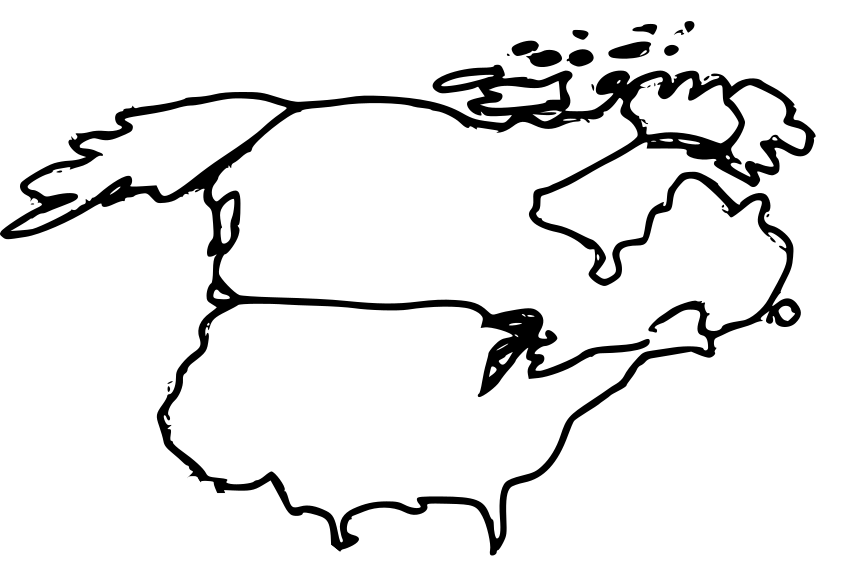
\includegraphics[width=1.5\textwidth]{imgs/usa.png}};
            %
            \draw[<-,very thick] ($(usa)+(1.9,-0.7)$) .. controls ($(usa)+(4.7,-0.4)$) .. ($(usa)+(5,0.1)$) node [above,align=center,font=\scriptsize] {\textbf{MIT}~\\ D. Bertsimas, R. Mazmuder, ...~\\\textit{Optimization tools for $\ell_0$-problems}};
        }
        %
        %
        %
        \onslide<3-> {
            \draw[<-,very thick] ($(usa)+(0.25,0.45)$) .. controls ($(usa)+(-1.9,0.1)$) .. ($(usa)+(-2.3,-0.1)$) node [below,align=center,font=\scriptsize] {\textbf{Google Deep Mind}~\\ H. Hazimeh, A. Dedieu, ...~\\\textit{MIP-based heuristics}};
            %
            \draw[<-,very thick] ($(usa)+(-0.5,-1.2)$) .. controls ($(usa)+(-1.5,-1.4)$) .. ($(usa)+(-2,-1.9)$) node [below,align=center,font=\scriptsize] {\textbf{Berkley}~\\ A. Atamtürk, A. Gomès, ...~\\\textit{Convex-based acceleration}};
        }
        %
        %
        %
        \onslide<4-> {
            \node[align=center,text width=0.3\linewidth] (europe) at ($(current page.center)+(3.75,-2.5)$) {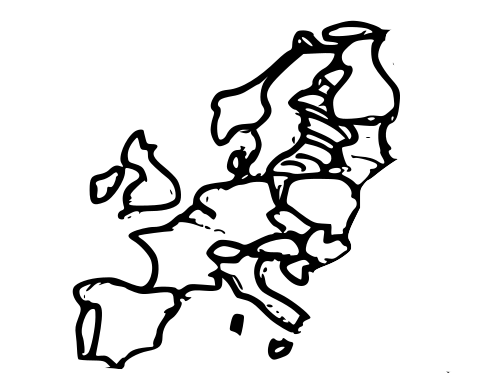
\includegraphics[width=1.5\textwidth]{imgs/europe.png}};
            %
            \draw[<-,very thick] ($(europe)+(0.7,1)$) .. controls ($(europe)+(0.5,1.5)$) .. ($(europe)+(1.1,3.5)$) node [above,align=center,font=\scriptsize] {\textbf{Lund University}~\\ M. Carlsson, C. Olsson...~\\\textit{Relaxation design}};
            %
            \draw[<-,very thick] ($(europe)+(0.4,0.1)$) .. controls ($(europe)+(-0.5,1.5)$) .. ($(europe)+(-1.2,2.5)$) node [above,align=center,font=\scriptsize] {\textbf{Frankfurt / Wurzburg Universities}~\\ C. Kanzow, A. Tillmann, ...~\\\textit{Optimality conditions}};
            %
            \draw[<-,very thick] ($(europe)+(-0.4,0.5)$) .. controls ($(europe)+(-1,1.3)$) .. ($(europe)+(-2,1.5)$) node [above left,align=center,font=\scriptsize] {\textbf{London Business School}~\\ J. Pauphilet, R. Cory-Wright, ...~\\\textit{Healthcare applications}};
        }
        %
        %
        %
        \onslide<5-> {
            \draw[<-,very thick] ($(europe)+(0.2,-0.6)$) .. controls ($(europe)+(-1.5,0.8)$) .. ($(europe)+(-2.5,0.9)$) node [left,align=center,font=\scriptsize] {\textbf{Ponts ParisTech}~\\ M. De Lara, P. Chancelier, A. Parmentier, ...~\\\textit{Non-convex analysis, ML appli.}};
            %
            \draw[<-,very thick] ($(europe)+(-0.4,-0.4)$) .. controls ($(europe)+(-1,-0.4)$) .. ($(europe)+(-5,-0.2)$) node [left,align=center,font=\scriptsize] {\textbf{Centrale Nantes / ENSTA Bretagne}~\\ S. Bourguignon, J. Ninin, ...~\\\textit{BnB with quadratic loss}};
            %
            \draw[<-,very thick] ($(europe)+(-0.2,-0.7)$) .. controls ($(europe)+(-4,-0.7)$) .. ($(europe)+(-5.7,-0.9)$) node [below left,align=center,font=\scriptsize] {\textbf{Inria / CentraleSupélec}~\\ C. Herzet, C. Elvira, A. Arslan, ...~\\\textit{Generic and efficient BnB}};
            %
            \draw[<-,very thick] ($(europe)+(0.1,-0.8)$) .. controls ($(europe)+(-0.5,-1.5)$) .. ($(europe)+(-1.7,-1.5)$) node [left,align=center,font=\scriptsize] {\textbf{IRIT / I3S}~\\ E. Soubies, L. Blanc-Féraud, ...~\\\textit{Convex-concave relaxation}};
        }
    \end{tikzpicture}
\end{frame}

\begin{frame}
    \begin{center}
        \Large{\textbf{Take-home messages}}
    \end{center}
    ~\\
    \begin{itemize}[label=\textbullet]
        \item Although \textcolor{TolLightOrange}{NP-hard}, $\ell_0$-problems are of \textcolor{TolLightOrange}{practical interest}
        \item There exists methods to tackle them
        \begin{itemize}[label=\textbullet]
        \item \textcolor{TolLightOrange}{MIP-based} formulation and generic solvers
        \item \textcolor{TolLightOrange}{BnB} algorithms with \textcolor{TolLightOrange}{specialized} steps
        \item \textcolor{TolLightOrange}{Structure-exploitation} is key
        \end{itemize}
        \item It's an active research area
        \begin{itemize}[label=\textbullet]
        \item Theoretical and methodological developments still needed
        \item Need to reach the applicative world
        \end{itemize}
    \end{itemize}
\end{frame}

\begin{frame}[standout]
  Question time ! ~\\~\\
  
\includegraphics[width=40pt]{imgs/nerd-face.png}
\end{frame}

\backupbegin
\begin{frame}{Compressed sensing}
    \begin{tikzpicture}[remember picture,overlay]
        \begin{scope}[xshift=0.5\textwidth]
            \onslide<1-> {
                \node[text width=0.25\linewidth,align=center] (groundtruth) at (-4,2.5) {Sparse signal \\ $\pv \in \kR^{\pdim}$};
                %
                \draw ($(groundtruth)+(0,-1.75)$) node {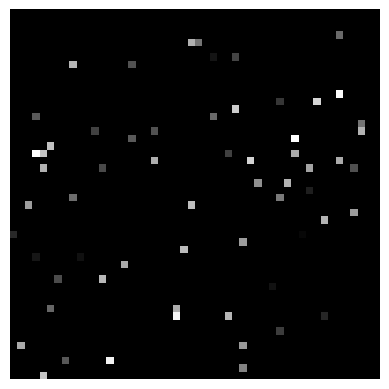
\includegraphics[width=2cm]{imgs/cs-x.png}};
                %
                \node at ($(groundtruth)+(0,-3)$) {$\pdim$ pixels};
            }
            %
            %
            %
            \onslide<2-> {
                \node[text width=0.25\linewidth,align=center] (observation) at (4,2.5) {Compressed signal \\ $\obs = \dic\pv \in \kR^{\ddim}$};
                %
                \draw[ultra thick,->] ($(groundtruth.north east)+(0,-0.25)$) .. controls (0,3.25) .. ($(observation.north west)+(0,-0.25)$) node[midway,fill=TolLightWhite,draw,ultra thick,text width=0.35\linewidth,align=center,yshift=-5] {Linear compression};
                %
                \draw ($(observation)+(0,-1.75)$) node {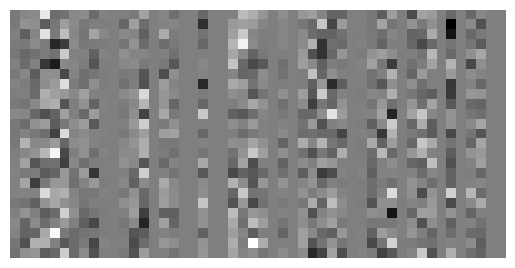
\includegraphics[width=2.5cm]{imgs/cs-y.png}};
                %
                \node at ($(observation)+(0,-2.75)$) {$\ddim$ pixels, $\ddim \ll \pdim$};
            }
            %
            %
            %
            \onslide<3-> {
                \draw[ultra thick,<-] ($(groundtruth.south east)+(0,0.25)$) .. controls (0,1.75) .. ($(observation.south west)+(0,0.25)$) node[midway,fill=TolLightWhite,draw,ultra thick,text width=0.35\linewidth,align=center,yshift=5] {Recover $\pv$ from $\dic$ and $\obs$};
            }
            %
            %
            %
            \onslide<4-> {
                \node [text width=0.45\textwidth] at (0,-1) (problem) {
                    \begin{blockcolor}{mDarkTeal}{Goal}
                    \centering
                    Find $\pv$ such that $\obs = \dic\pv$
                    \end{blockcolor}
                };
            }
            %
            %
            %
            \onslide<5-> {
                \node [text width=0.45\textwidth] at ($(problem)+(0,-2.25)$) (problem-sparse) {
                    \begin{blockcolor}{mDarkTeal}{Goal}
                        \centering
                        Find $\pv$ \textcolor{TolLightOrange}{sparse} such that $\obs = \dic\pv$
                    \end{blockcolor}
                };
                %
                \draw[ultra thick,->] ($(problem)+(0,-0.75)$) -- ($(problem-sparse)+(0,0.5)$) node[midway,fill=TolLightWhite,draw,ultra thick] {no unique solution};
            }
        \end{scope}
    \end{tikzpicture}
\end{frame}
  
\begin{frame}{Feature selection}
    \begin{tikzpicture}[remember picture,overlay]
        \begin{scope}[xshift=0.5\textwidth]
            \onslide<1-> {
                \node (table) at (0,1.5) {
                    \begin{tabular}{c|cccc|c}
                        \toprule
                        & \textbf{Feature 1} & \textbf{Feature 2} & $\quad$...$\quad$ & \textbf{Feature n} & $\ \ $\textbf{Target}$\ \ $ \\
                        \midrule
                        \textbf{Sample 1} & \textcolor{mDarkTeal!20}{$a_{1,1}$} & \textcolor{mDarkTeal!20}{$a_{1,2}$} & \textcolor{mDarkTeal!20}{...} & \textcolor{mDarkTeal!20}{$a_{1,\pdim}$} & \textcolor{mDarkTeal!20}{$\obsi{1}$} \\
                        \textbf{Sample 2} & \textcolor{mDarkTeal!20}{$a_{2,1}$} & \textcolor{mDarkTeal!20}{$a_{2,2}$} & \textcolor{mDarkTeal!20}{...} & \textcolor{mDarkTeal!20}{$a_{2,\pdim}$} & \textcolor{mDarkTeal!20}{$\obsi{2}$} \\
                        \textbf{Sample 3} & \textcolor{mDarkTeal!20}{$a_{3,1}$} & \textcolor{mDarkTeal!20}{$a_{3,2}$} & \textcolor{mDarkTeal!20}{...} & \textcolor{mDarkTeal!20}{$a_{3,\pdim}$} & \textcolor{mDarkTeal!20}{$\obsi{3}$} \\
                        \textcolor{mDarkTeal!20}{...} & \textcolor{mDarkTeal!20}{...} & \textcolor{mDarkTeal!20}{...} & \textcolor{mDarkTeal!20}{...} & \textcolor{mDarkTeal!20}{...} & \textcolor{mDarkTeal!20}{...} \\
                        \textbf{Sample m} & \textcolor{mDarkTeal!20}{$a_{\ddim,1}$} & \textcolor{mDarkTeal!20}{$a_{\ddim,2}$} & \textcolor{mDarkTeal!20}{...} & \textcolor{mDarkTeal!20}{$a_{\ddim,\pdim}$} & \textcolor{mDarkTeal!20}{$\obsi{\ddim}$} \\
                        \bottomrule
                    \end{tabular}
                };
                %
                \node[draw,ultra thick,fill=TolLightWhite,font=\small] (features) at ($(table.center)+(0,-0.5)$) {$\dic \in \kR^{\ddim\times\pdim}$};
                \node[draw,ultra thick,fill=TolLightWhite,font=\small] (outcome) at ($(table.center)+(4.2,-0.5)$) {$\obs \in \kR^{\ddim}$};
            }
            %
            %
            %
            \onslide<2-> {
                \node[text width=0.275\linewidth,align=center] (feature) at ($(table.south)+(-3.5,-0.6)$) {Features $\dic \in \kR^{\ddim\times\pdim}$};
                \node[text width=0.275\linewidth,align=center] (outcome) at ($(table.south)+(3.5,-0.6)$) {Target $\obs = \phi(\dic\pv)$};
                %
                \draw[ultra thick,<->] (feature) -- (outcome) node[midway,below,TolLightOrange] {weights $\pv \in \kR^{\pdim}$};
            }
            %
            %
            %
            \onslide<3-> {
                \node[font=\small,text width=0.3\linewidth,align=center] (loss) at ($(table.south)+(-1.75,-2)$) {\textbf{Model accuracy} \\ Loss $\mathcal{L}_{\phi}(\dic\pv,\obs)$};
                %
                \node[font=\small,text width=0.3\linewidth,align=center] (reg) at ($(table.south)+(1.75,-2)$) {\textbf{Model explainability} \\ Use few features};
            }
            %
            %
            %
            \onslide<4-> {
                \draw[ultra thick,->] (loss) -- ($(loss)+(0,-0.75)$);
                \draw[ultra thick,->] (reg) -- ($(reg)+(0,-0.75)$);
                %
                \node[align=center,text width=0.6\textwidth] (serm) at ($(table.south)+(0,-3.25)$) {
                    \begin{blockcolor}{mDarkTeal}{Goal}
                    \centering
                    Find $\pv$ \textcolor{TolLightOrange}{sparse} such that $\mathcal{L}_{\phi}(\dic\pv,\obs)$ is small 
                    \end{blockcolor}
                };
            }
        \end{scope}
    \end{tikzpicture}
\end{frame}
  
\begin{frame}{Network design}
    \begin{tikzpicture}[remember picture,overlay]
        \begin{scope}[xshift=0.5\textwidth]
            \onslide<1-> {
                \coordinate (A) at (-3.5,1);
                \coordinate (B) at ($(A)+(2,0)$);
                \coordinate (C) at ($(A)+(1,2)$);
                \coordinate (D) at ($(A)+(1,-2)$);
                \coordinate (E) at ($(A)+(3,1)$);
                \coordinate (F) at ($(A)+(3,-1)$);
                \coordinate (G) at ($(A)+(-1,1.5)$);
                \coordinate (H) at ($(A)+(-1,-1.5)$);
                \coordinate (I) at ($(A)+(4,0)$);
                \coordinate (J) at ($(A)+(-2,0)$);

                \draw[ultra thick,dashed] (A) -- (B);
                \draw[ultra thick,dashed] (A) -- (C);
                \draw[ultra thick,dashed] (A) -- (D);
                \draw[ultra thick,dashed] (A) -- (G);
                \draw[ultra thick,dashed] (A) -- (H);
                \draw[ultra thick,dashed] (B) -- (C);
                \draw[ultra thick,dashed] (B) -- (D);
                \draw[ultra thick,dashed] (B) -- (E);
                \draw[ultra thick,dashed] (B) -- (F);
                \draw[ultra thick,dashed] (B) -- (I);
                \draw[ultra thick,dashed] (C) -- (E);
                \draw[ultra thick,dashed] (C) -- (G);
                \draw[ultra thick,dashed] (D) -- (F);
                \draw[ultra thick,dashed] (D) -- (H);
                \draw[ultra thick,dashed] (E) -- (I);
                \draw[ultra thick,dashed] (F) -- (I);
                \draw[ultra thick,dashed] (G) -- (H);
                \draw[ultra thick,dashed] (G) -- (J);
                \draw[ultra thick,dashed] (H) -- (J);

                \node[ultra thick, circle, draw, minimum size=6mm, fill=TolLightWhite] at (A) {};
                \node[ultra thick, circle, draw, minimum size=6mm, fill=TolLightWhite] at (B) {};
                \node[ultra thick, circle, draw, minimum size=6mm, TolLightRed, fill=TolLightWhite] at (C) {\small\textcolor{TolLightRed}{\textbf{3}}};
                \node[ultra thick, circle, draw, minimum size=6mm, TolLightRed, fill=TolLightWhite] at (D) {\small\textcolor{TolLightRed}{\textbf{3}}};
                \node[ultra thick, circle, draw, minimum size=6mm, fill=TolLightWhite] at (E) {};
                \node[ultra thick, circle, draw, minimum size=6mm, fill=TolLightWhite] at (F) {};
                \node[ultra thick, circle, draw, minimum size=6mm, fill=TolLightWhite] at (G) {};
                \node[ultra thick, circle, draw, minimum size=6mm, fill=TolLightWhite] at (H) {};
                \node[ultra thick, circle, draw, minimum size=6mm, TolLightRed, fill=TolLightWhite] at (I) {\small\textcolor{TolLightRed}{\textbf{3}}};
                \node[ultra thick, circle, draw, minimum size=6mm, TolLightBlue, fill=TolLightWhite] at (J) {\small\textcolor{TolLightBlue}{\textbf{9}}};

                \node[text width=0.6\linewidth,align=center] at (-2.5,-2) {Which edges to build to transport products from \textcolor{TolLightBlue}{source} to \textcolor{TolLightRed}{sink} nodes ?};
            }
            %
            %
            %
            \onslide<2-> {
                \node[ultra thick, circle, draw, minimum size=6mm, fill=TolLightWhite] (N1) at (2.25,3) {};
                \node[ultra thick, circle, draw, minimum size=6mm, fill=TolLightWhite] (N2) at (4.75,3) {};
                \draw[ultra thick,dashed] (N1) -- (N2) node[midway,above,font=\small] {edge $\idxentry \in I$} node[midway,below,font=\small] {flow $\pvi{\idxentry} \geq 0$};
            }
            %
            %
            %
            \onslide<3-> {
                \node[text width=0.5\linewidth,align=center,anchor=north] at ($(N1)!0.5!(N2)+(0,-0.75)$) {construct edge $\idxentry \in I$ if $\pvi{\idxentry} > 0$ \\ \textcolor{TolLightOrange}{pay construction cost $c$}};
            }
            %
            %
            %
            \onslide<4-> {
                \node[text width=0.4\linewidth,align=center,anchor=north] at ($(N1)!0.5!(N2)+(0,-2.5)$) {\textbf{Question} \\ How to construct the least number of edges to satisfy transportation needs ?};
            }
            %
            %
            %
            \onslide<5-> {
                \node[text width=0.45\linewidth,align=center,anchor=north] at ($(N1)!0.5!(N2)+(0,-5.25)$) {Find $\pv \in \kR^{\card(I)}$ \textcolor{TolLightOrange}{sparse} such that $\mathcal{Q}(\pv)$ $=$ $0$};
                %
                \draw[ultra thick,<->] ($(N1)!0.5!(N2)+(0,-4.5)$) -- ($(N1)!0.5!(N2)+(0,-5.25)$);
            }
        \end{scope}
    \end{tikzpicture}
\end{frame}

\begin{frame}{Balancing solution quality and problem hardness}
    \begin{tikzpicture}[remember picture,overlay]
        \onslide<1-> {
            \begin{scope}[xshift=0.5\textwidth]
                \node (dataset) at (0,2.5) {
                    \scriptsize
                    \begin{tabular}{c|cccccc|c}
                        \multicolumn{8}{c}{\small{Riboflavin dataset - P. Bühlmann \textit{et al.} (2014)}} \\
                        \toprule
                        Colony & AADK & AAPA & ABFA & ABH & ... & ZUR & \textbf{B2 prod.} \\
                        \midrule
                        \#1 & 8.49 & 8.11 & 8.32 & 10.28 & ... & 7.42 & \textbf{-6.64} \\
                        \#2 & 7.29 & 6.39 & 11.32 & 9.42 & ... & 6.99 & \textbf{-5.43} \\
                        ... & ... & ... & ... & ... & ... & ... & ... \\
                        \#71 & 6.85 & 8.27 & 7.98 & 8.04 & ... & 6.65 & \textbf{-7.58} \\
                        \bottomrule
                    \end{tabular}
                };
                %
                \draw[very thick] ($(dataset.south)+(-2.4,0)$) -- ($(dataset.south)+(-2.4,-0.1)$) -- ($(dataset.south)+(2.15,-0.1)$) node[midway,below,font=\small] {4,088 genes} -- ($(dataset.south)+(2.15,0)$);
            \end{scope}
        }
        %
        %
        %
        \onslide<2-> {
            \begin{scope}[xshift=30,yshift=-80]
                \pgfplotscreateplotcyclelist{cycle_quality_hardness}{
                    TolLightBlue, very thick, mark=*, mark options={scale=0.5}\\
                    TolLightBrown, very thick, mark=*, mark options={scale=0.5}\\    
                    TolLightRed, very thick, mark=*, mark options={scale=0.5}\\
                }
                \begin{groupplot}[
                    group style={
                        group size=2 by 1,
                        horizontal sep=0.2\textwidth,
                    },
                    width   = 0.48\textwidth,
                    height  = 0.4\textwidth,
                    xlabel  = \textbf{Number of genes},
                    legend columns=5, 
                    legend style={
                        at={(-0.35,1)},
                        anchor=south,
                        /tikz/every even column/.style = {column sep=5pt},
                        draw=none,
                    },
                    cycle list name=cycle_quality_hardness,
                    mbaseplot,
                    axis line style = ultra thick,
                    major tick style = {ultra thick,color=mDarkTeal},
                    minor tick style={draw=none},
                    xmajorgrids=true,
                    ymajorgrids=true,
                    major grid style={dotted},
                    axis x line=bottom,
                    axis y line=left,
                ]

                    \nextgroupplot[
                        ylabel = \textbf{Model error},
                        ymode=log,
                        ymin=0.09,
                        ymax=1.5,
                    ]
                    \foreach \method in {omp,lasso,el0ps} {
                        \addplot table[x=nnz_grid,y=\method_test_error,col sep=comma]{data/riboflavin_quality.csv};
                    }

                    \nextgroupplot[
                        ymode=log,
                        ylabel = \textbf{Time (sec.)},
                        ytick={0.001,0.01,0.1,1,10,100},
                        ymax=500,
                        ymin=0.0004,
                    ]
                    \foreach \method in {omp,lasso,l0bnb} {
                        \addplot table[x=nnz_grid,y=\method_solve_time,col sep=comma]{data/riboflavin_quality.csv};
                    }

                    \addlegendentry{Omp (heuristic)};
                    \addlegendentry{Lasso (convex problem)};
                    \addlegendentry{$\ell_0$-problem (np-hard problem)};
                \end{groupplot}
            \end{scope}
        }
    \end{tikzpicture}
\end{frame}
\backupend

\end{document}
